%==============================================================================
% Forecasting quarterly short-term-rental demand from public availability
% snapshots -- 2025-2026 New York City Inside Airbnb data.
% Standalone, double-blind IEEE journal manuscript.
% Build:  pandoc main_p2.tex -> docx  ->  build_paper2.py  ->  Word/PDF
%         (or upload the paper2/ folder to Overleaf and compile main_p2.tex)
%==============================================================================
\documentclass[journal]{IEEEtran}
\usepackage{amsmath,amssymb,amsfonts}
\usepackage{graphicx}
\usepackage{textcomp}
\usepackage{booktabs}
\usepackage{url}
\usepackage[T1]{fontenc}
\usepackage[utf8]{inputenc}
\usepackage{xcolor}
\graphicspath{{figures/}}
\hyphenation{short-term}

\begin{document}

\title{Forecasting Quarterly Short-Term-Rental Demand from Public Availability
Snapshots: A Leakage-Safe Convex Ensemble on 2025--2026 New York City Data}

\author{Anonymous Author(s)%
\thanks{Author names and affiliations omitted for double-blind review.}}

\markboth{Manuscript submitted for review}%
{Forecasting Quarterly Short-Term-Rental Demand from Public Availability Snapshots}
\maketitle

\begin{abstract}
Accurately forecasting how heavily a short-term rental will be booked is valuable
for hosts, platforms, and municipal regulators, yet most public data expose only
coarse calendar availability rather than an explicit booking record. This paper
studies quarterly demand forecasting for New York City short-term rentals using
ten consecutive monthly Inside Airbnb snapshots (July 2025--April 2026). Because
the calendars provide only an \texttt{available} (true/false) flag and no usable
price, the prediction target---booked nights in a future quarter---is reconstructed
by \emph{snapshot differencing}: a date that transitions from available to
unavailable across consecutive snapshots, and stays unavailable, is counted as
booked. The resulting target is a censored, zero-inflated integer in $[0,92]$ with
roughly half its mass at zero. A single leakage-safe pipeline---median imputation,
one-hot encoding, and a $K$-fold target encoder for high-cardinality location
fields---feeds six learners (Linear Regression, Random Forest, XGBoost, LightGBM,
CatBoost, and a PyTorch multi-layer perceptron trained with Adam) that are combined
by a convex weighted blend whose weights are found by
Sequential Least-Squares Quadratic Programming (SLSQP). Using a seven-month
behavioural history to predict the February--April 2026 quarter, the blend attains
a $20\%$ held-out test $R^2$ of $0.654$, within $0.011$ of its cross-validation
estimate, and the improvement over the best single learner is statistically
significant. The method is validated across three independent target quarters,
and a controlled ablation shows that the dominant lever is the target definition
and the depth of behavioural history; hyper-parameter tuning, a two-stage hurdle
model, enriched price features, and review-velocity features each add little or
nothing. The results indicate that the achievable accuracy on this public data
source is bounded primarily by label quality rather than by model capacity.
\end{abstract}

\begin{IEEEkeywords}
Short-term rental, demand forecasting, Inside Airbnb, zero-inflated regression,
gradient boosting, target encoding, model blending, convex optimization,
snapshot differencing, censored data.
\end{IEEEkeywords}

%==============================================================================
\section{Introduction}
\IEEEPARstart{S}{hort-term} rental (STR) platforms such as Airbnb have reshaped
urban accommodation, and the volume of nights a listing will be booked over a
future period is one of the most consequential quantities in the ecosystem. A
host who anticipates a busy quarter can schedule maintenance, adjust pricing, and
plan staffing; a platform can allocate customer-support and marketing resources
toward listings likely to be under-booked; and a municipality can use aggregate
booking-density estimates to study the pressure that short-term letting places on
long-term housing supply. All three applications require a quantitative,
per-listing forecast of future demand rather than a qualitative signal.

These three constituencies value the forecast for different but complementary
reasons. For an individual \emph{host}, a quarter-ahead estimate of occupancy
translates directly into operational decisions: whether to raise nightly rates for
an anticipated peak, when to schedule cleaning and maintenance around expected
gaps, and whether the projected revenue justifies hiring help or investing in the
property. For the \emph{platform}, aggregating per-listing forecasts across a city
yields a demand map that informs where to concentrate customer-support capacity
before a busy period, which under-booked listings to surface in search or target
with promotions, and how to calibrate the pricing recommendations shown to hosts.
For a \emph{municipality} or housing researcher, booking-density estimates provide
an evidence base for studying how intensively the short-term-rental stock is used
and, by extension, how much long-term housing it displaces---a question of active
policy interest in dense markets such as New York City. In all three cases the
useful object is a calibrated numerical prediction for each individual listing,
which is the quantity this paper targets.

Two structural properties make this forecasting problem hard. First, demand is a
\emph{censored count}: a listing can be booked for anywhere between zero and the
number of nights in the quarter, and the observed value saturates at both ends.
Second, and more importantly for real data, the demand distribution is heavily
\emph{zero-inflated}: in the market studied here roughly half of all listings are
booked for zero nights in the target quarter, reflecting the large population of
dormant or seasonally inactive listings that characterises the post-regulation New
York City market. A forecaster must therefore predict a spike of zeros, a long
right tail, and a pile-up at the upper bound simultaneously.

The New York City market adds a further layer of difficulty that is characteristic
of the current regulatory era. Following the enforcement of strict short-term
registration rules, a large share of listings became dormant or permanently
blocked, so the population is a mixture of genuinely active rentals and a long tail
of inactive shells. A forecaster must therefore simultaneously recognise which
listings are effectively out of the market---a near-deterministic zero---and, for
the active remainder, predict a continuous, right-skewed count. This mixture is
precisely what produces the sharp zero spike observed in the target and what makes
a naive occupancy count so misleading.

A further, and often under-appreciated, difficulty concerns the \emph{data source}
itself. Much of the academic literature on STR modelling is built on the 2016-era
scrape formats, which record an explicit per-day booking status and a per-day
price. Contemporary public snapshots---most prominently those distributed by the
Inside Airbnb project \cite{insideairbnb}---have converged on a much coarser
format: the daily calendar exposes only a Boolean \texttt{available} field
(true/false), with no explicit ``booked'' status, and, as we document in
Section~\ref{sec:data}, the calendar price field has become empty in recent
snapshots. Consequently a modern demand study cannot simply read a booking label;
it must \emph{reconstruct} the target from the way availability evolves over time,
and it loses the strong price-dynamics signal that earlier work relied upon.

\emph{Research gap.} While tree-based ensembles are firmly established for
STR \emph{price} prediction, systematic, leakage-safe frameworks that forecast
per-listing \emph{demand} directly from modern, coarse public availability
snapshots---jointly handling extreme zero-inflation, a hard bounded support, and a
target that must be recovered by differencing rather than read off---remain
under-explored. In particular, it is unclear how much predictive accuracy is
attainable from such data, and whether the residual error is driven by the model
or by the data itself.

\emph{Contributions.} This paper makes the following contributions.
\begin{itemize}
\item It formalises a \emph{snapshot-differencing} construction of the demand
target from Boolean availability calendars, and shows empirically that it yields a
zero-inflated, bounded booking signal, whereas the naive occupancy proxy is
dominated by host blocking and is therefore unsuitable.
\item It presents a single leakage-safe pipeline---median imputation, one-hot and
$K$-fold target encoding, six heterogeneous learners, and an SLSQP convex
blend---and evaluates it with both cross-validation and a disjoint held-out test
set, reaching a held-out $R^2$ of $0.654$.
\item It validates the method across three independent target quarters, providing
evidence of temporal robustness.
\item It reports a controlled ablation that isolates the contribution of every
design choice and yields several honest \emph{negative} findings: posted price
does not predict demand in this market, review-velocity features are redundant
with calendar-derived activity, and an explicit two-stage hurdle model does not
improve on the direct blend.
\end{itemize}

The remainder of the paper is organised as follows.
Section~\ref{sec:related} reviews related work. Section~\ref{sec:data} describes
the data and the target construction. Section~\ref{sec:method} details the
methodology. Section~\ref{sec:results} reports results, and
Section~\ref{sec:ablation} the ablation study. Section~\ref{sec:limits} discusses
limitations and future work, and Section~\ref{sec:concl} concludes.

A guiding principle throughout is that every reported number should be defensible
as an estimate of genuinely out-of-sample performance. This shapes several choices
that might otherwise seem conservative: the exclusion of forward-looking
availability fields even though they are highly predictive, the reconstruction of
the target from history alone, the use of a disjoint held-out test set in addition
to cross-validation, and the validation of the same pipeline across multiple
quarters. The consequence is a headline accuracy that is lower than a leakage-prone
or single-split study might report, but that can be trusted as a realistic estimate
of what the method would achieve on future listings---which is the only accuracy
that matters for the operational applications described above.

%==============================================================================
\section{Related Work}
\label{sec:related}
We organise related work into five threads.

\subsection{Machine learning for short-term-rental prediction}
A substantial body of work applies machine learning to Airbnb data, predominantly
for price prediction. Tang, Cheng, and Zhang \cite{tang2024} compared ten
algorithms on Sydney listings and found gradient-boosted trees, and CatBoost in
particular, to be strongest. Camatti et al.\ \cite{camatti2024} contrasted
artificial-intelligence and traditional methods on Dutch listings and observed
that tree-based and neural approaches overfit less than linear regression.
Rezazadeh Kalehbasti et al.\ \cite{kalehbasti2019} predicted New York City prices
from property attributes, host characteristics, and review sentiment. Islam et
al.\ \cite{islam2022} combined a topic model over descriptions with an XGBoost
regressor. Two lessons recur across this literature and inform the present work:
the most useful predictors mix structural attributes, location, and dynamic
calendar or review information; and gradient-boosted trees are a strong default on
the mixed numerical/categorical tables that describe rentals. A second, quieter
theme in this literature is methodological: many studies report a single
cross-validation score on a single city and period, without a disjoint held-out
test or an out-of-time check, which makes it difficult to know how much of the
reported accuracy would survive on genuinely unseen data. A recurring concern is
also leakage---features derived from the same period as the target, or forward
-looking availability fields that encode the answer---which can silently inflate
results. The present work addresses both concerns directly, with an explicit
held-out test set, validation across three independent quarters, and a feature
construction that is leakage-safe by design.

\subsection{Decision trees and gradient boosting}
The decision tree \cite{quinlan1986} yields interpretable, non-parametric
regressors, but a single tree overfits. Bagging \cite{breiman1996} and Random
Forests \cite{breiman2001} reduce variance by averaging decorrelated trees, while
gradient boosting \cite{friedman2001} reduces bias by fitting residuals
sequentially. XGBoost \cite{chen2016xgboost}, LightGBM \cite{ke2017lightgbm}, and
CatBoost \cite{prokhorenkova2018catboost} are widely used, highly optimised
implementations with regularisation, sparsity-aware splitting, and efficient
categorical handling; all three are used here as base learners. Their inductive biases differ enough to
make them useful ensemble members: Random Forest reduces variance through bagging
and random feature selection but cannot reduce bias as aggressively as boosting;
gradient boosting attains low bias through sequential residual fitting but must be
regularised to control the corresponding variance; and the three boosting
implementations differ in their split-finding, leaf-growth, and categorical-handling
strategies, so their errors are correlated but not identical---the property a blend
exploits. A linear model, though far weaker on this non-linear target, provides an
interpretable reference and occasionally contributes a small, complementary signal
to the blend.

\subsection{Leakage-safe preprocessing and target encoding}
Careful preprocessing---imputation, encoding, and, above all, preventing leakage
by fitting every transform inside the training fold---has a large effect on the
final error \cite{pedregosa2011sklearn}. High-cardinality categoricals such as
neighbourhood are commonly handled by target (mean) encoding; a leakage-aware
variant computes the encoding inside an inner cross-validation loop so that no row
informs its own encoded value. We adopt this $K$-fold target encoder with additive
smoothing. Target encoding is particularly appropriate for a field such as
neighbourhood, which has hundreds of levels of very uneven frequency: one-hot
encoding would produce a wide, sparse matrix and treat every neighbourhood as
equidistant, whereas a smoothed mean encoding places each neighbourhood on a single
demand-relevant axis and gracefully shrinks rare levels toward the global mean. The
additive-smoothing parameter controls this shrinkage, and the inner
cross-validation loop is what prevents the well-known optimism that naive mean
encoding introduces when a row is allowed to see its own label.

\subsection{Model blending and stacking}
Rather than selecting a single estimator, combining several models often improves
accuracy. Stacked generalisation \cite{wolpert1992stacked} learns a meta-model
over base predictions; a simpler and more robust variant constrains the
combination to a convex weighting of the base learners. We use the latter,
optimising the weights on out-of-fold predictions. The convex constraint is not
merely a computational convenience: by forcing the weights onto the probability
simplex it guarantees that the blended prediction remains on the same scale and
within the same support as its inputs, prevents any single learner from dominating
through an unbounded coefficient, and acts as a strong regulariser that makes the
learned weights stable across resampling. In our experiments an unconstrained
least-squares stack was no more accurate and considerably less stable than the
convex blend, which is why the constrained formulation is adopted throughout.

\subsection{Zero-inflated targets and occupancy estimation}
Count targets with excess zeros motivate dedicated models: zero-inflated and
hurdle (two-part) models separate the ``is it booked at all'' decision from the
positive count, and censored-regression estimators such as Tobit \cite{tobin1958}
treat the bound explicitly. Dietterich \cite{dietterich1998} recommends paired
resampling tests for comparing learners, which we adopt. The blending literature also cautions that combining models is not automatically
beneficial: an equal-weight average can be dragged down by weak members and an
unconstrained stack can overfit at the meta-level. The convex formulation used here
sits between these extremes, and part of the contribution of this paper is to
demonstrate, on a concrete large-scale problem, that the constrained blend delivers
a small but statistically reliable gain whereas the naive average does not.
Because Inside Airbnb
exposes no booking label, prior work has estimated occupancy either from
review activity (the ``San Francisco model'') or from availability changes; the
present paper uses the latter, formalised as snapshot differencing, and evaluates
a hurdle model as an ablation. The occupancy-estimation approaches are worth
situating. The review-based method infers nights booked from the number of reviews,
a review rate, and an assumed average stay; it is simple but rests on strong
assumptions and inherits the sparsity of reviews. The availability-change approach
adopted here makes fewer distributional assumptions and uses the calendar directly,
but must contend with the ambiguity between booking and blocking. Neither recovers a
perfect label, and the choice between them is a bias--variance trade-off: the
differencing target is a low-assumption estimator whose residual bias is the
host-blocking contamination that the multi-snapshot transition rule is designed to
suppress.

%==============================================================================
\section{Data and Problem Setting}
\label{sec:data}
\subsection{Data source and snapshots}
The study uses public Inside Airbnb snapshots \cite{insideairbnb} for New York
City. Ten consecutive monthly snapshots are available, spanning July 2025 through
April 2026. Each snapshot contains a \texttt{listings} table (per-property
attributes: property and room type, capacity, bedrooms and bathrooms, host flags,
review counts and scores, neighbourhood, latitude/longitude, amenities, and more),
a \texttt{calendar} table (one row per listing per future date, holding a Boolean
\texttt{available} field and, in principle, a price), and a \texttt{reviews} table
(one row per review, with its date). Each calendar looks forward roughly 365 days
from the scrape date. Table~\ref{tab:snapshots} summarises the snapshots.

The forward-looking nature of the calendar is essential to understanding both the
target construction and the leakage constraints. A snapshot scraped in a given
month contains, for each listing, the availability of every date from the scrape
date up to roughly one year ahead; it contains no past dates. A future date such as
one in February 2026 therefore appears as a forward entry in every snapshot from
mid-2025 onward and disappears from the calendars once it has passed. Observing the
same future date across the sequence of snapshots is what makes differencing
possible, and it also delimits which target quarters are recoverable: a quarter can
be reconstructed only if the snapshots that still contain its dates as future
entries are available. The ten-month window used here supports the three setups of
Table~\ref{tab:setups}, of which the February--April 2026 quarter admits the
deepest usable history.

\begin{table}[!t]
\caption{Monthly Inside Airbnb snapshots used (New York City).}
\label{tab:snapshots}
\centering
\small
\begin{tabular}{lll}
\toprule
Snapshot & Calendar forward span & Notes \\
\midrule
Jul--Nov 2025 & $\sim$365 days & price field $\approx$59\% populated \\
Dec 2025 & $\sim$365 days & price field empty \\
Jan--Feb 2026 & $\sim$365 days & price field empty \\
Mar--Apr 2026 & $\sim$365 days & no price column at all \\
\bottomrule
\end{tabular}
\end{table}

\subsection{Two data-quality findings}
Two properties of the modern format shape the entire study. First, the calendar's
\texttt{available} field is Boolean: \texttt{f} means the date is \emph{not}
bookable, but this conflates guest bookings with host-initiated blocking. As
Fig.~\ref{fig:avail} shows, roughly $77\%$ of calendar-days are unavailable,
consistent with a market in which many listings are dormant or heavily blocked.
Second, the per-day price signal has degraded: as Fig.~\ref{fig:price} shows, the
\texttt{listings} price is populated for only about $59\%$ of listings in the
months that retain it, and is entirely empty in the December~2025--February~2026
snapshots, while the March and April 2026 calendars drop the price column
altogether. The daily price-dynamics signal that earlier STR studies exploited is
therefore unavailable here. These two degradations are not incidental quirks of a
single download but reflect a broader trajectory in which the public data have
become progressively less granular over time; a study built on contemporary
snapshots must therefore be designed around their absence rather than assuming the
richer fields of earlier formats. The methodological response adopted here---
reconstructing the label by differencing and abandoning price as a predictor---is a
direct consequence of these constraints, and the resulting accuracy should be read
in that light: it is the accuracy attainable from what the modern public data
actually provide, not from an idealised record.

\begin{figure}[!t]
\centering
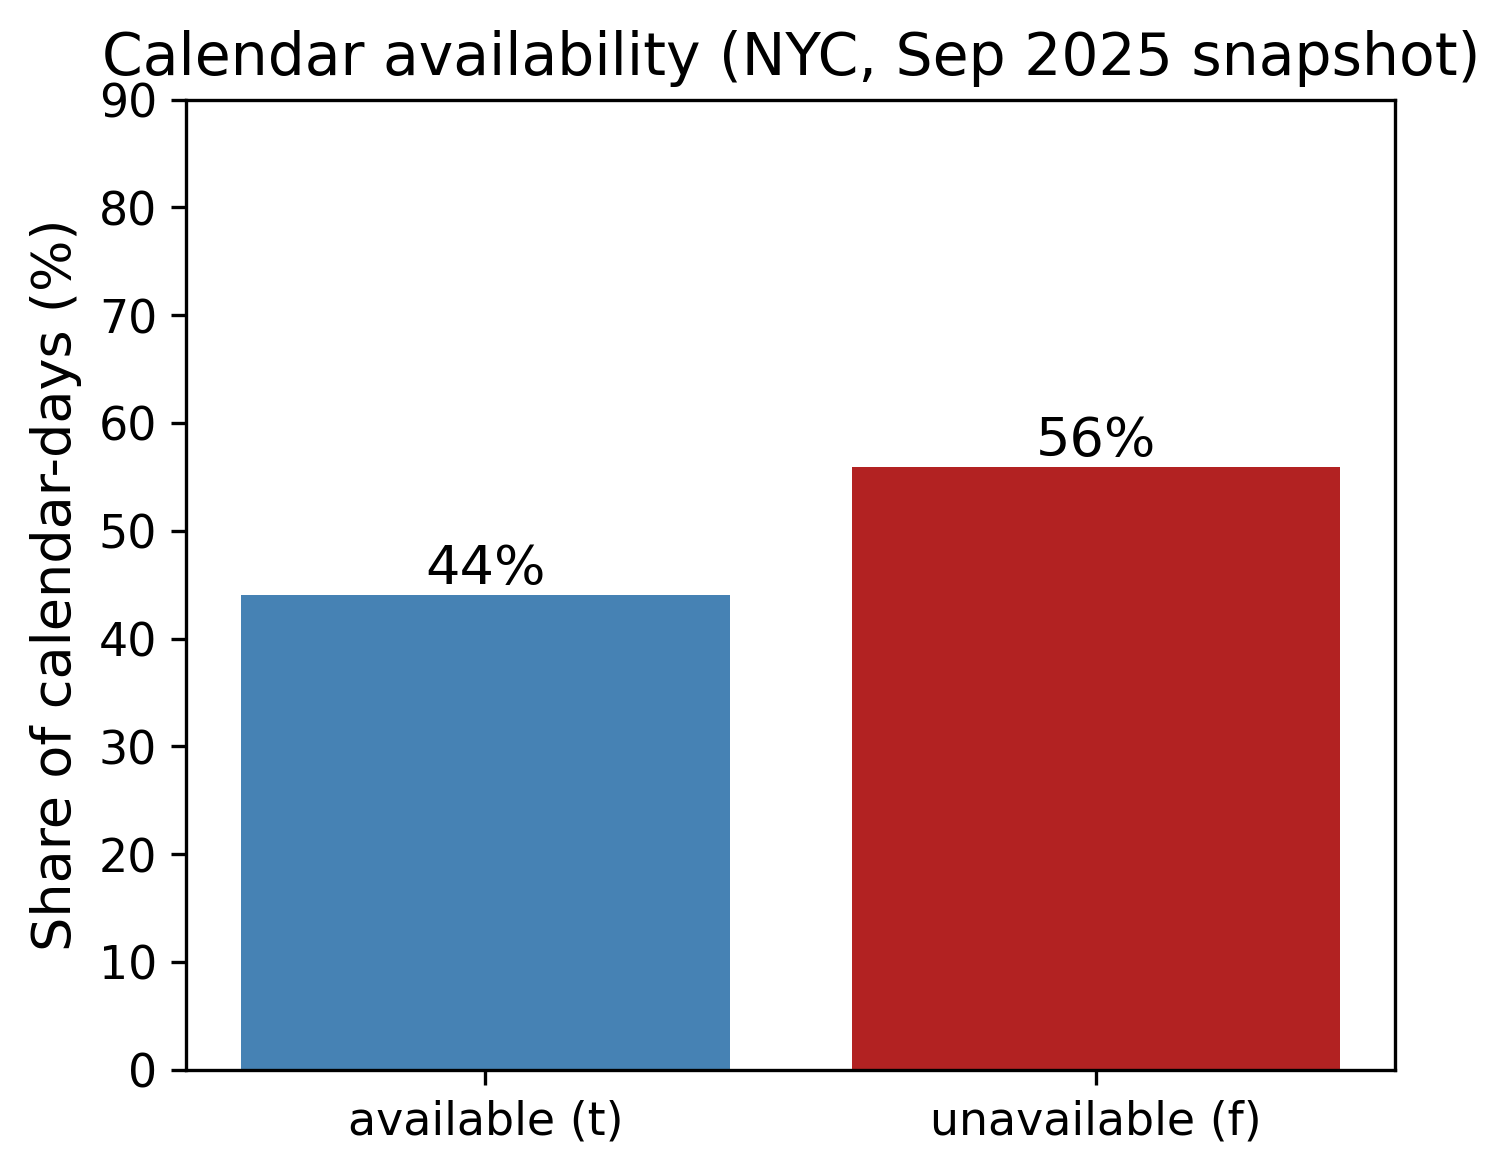
\includegraphics[width=\columnwidth]{fig2_availability.png}
\caption{Calendar availability. About $77\%$ of calendar-days are unavailable,
reflecting heavy host blocking and dormancy; the raw ``unavailable'' count is
therefore a poor proxy for realised demand.}
\label{fig:avail}
\end{figure}

\begin{figure}[!t]
\centering
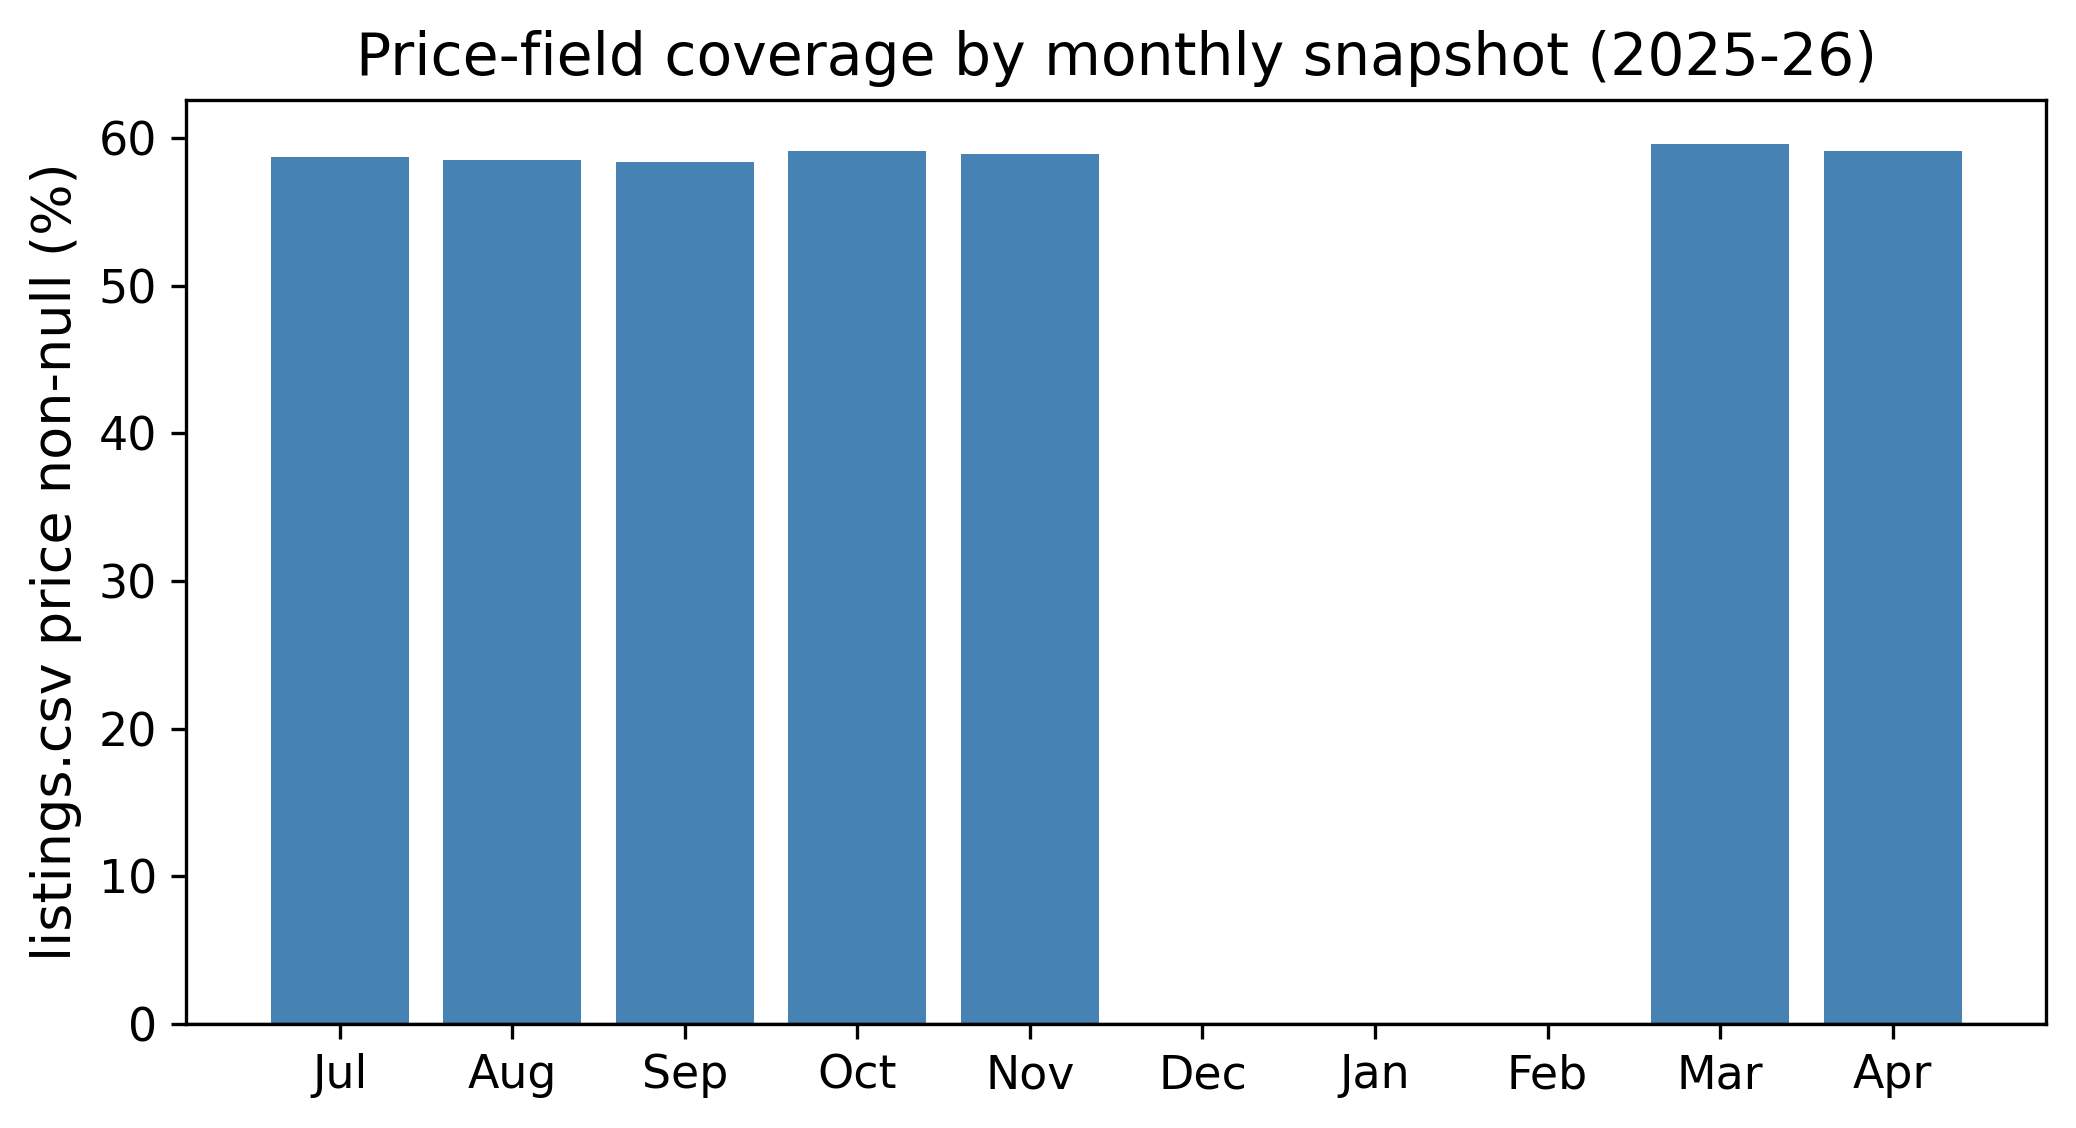
\includegraphics[width=\columnwidth]{fig3_price_coverage.png}
\caption{Price-field coverage by monthly snapshot. Price is $\approx$59\%
populated in some months and entirely absent in others, precluding a reliable
price-dynamics feature.}
\label{fig:price}
\end{figure}

Beyond price, several \texttt{listings} fields are substantially incomplete, as
summarised in Table~\ref{tab:missing}. Host-responsiveness fields and free-text
descriptions are missing for a large fraction of listings, so the pipeline encodes
missingness explicitly (median imputation with indicator flags) rather than
discarding these rows, because missingness itself is informative---an absent
response rate typically marks an inactive host.

\begin{table}[!t]
\caption{Missing-value rates of selected \texttt{listings} fields
(September 2025 snapshot).}
\label{tab:missing}
\centering
\small
\begin{tabular}{lc}
\toprule
Field & Missing rate \\
\midrule
\texttt{neighborhood\_overview} & 47.9\% \\
\texttt{host\_about} & 45.5\% \\
\texttt{host\_response\_rate} & 43.2\% \\
\texttt{host\_acceptance\_rate} & 43.0\% \\
\texttt{host\_location} & 24.0\% \\
\bottomrule
\end{tabular}
\end{table}

\subsection{Auxiliary review signal}
The reviews table provides an independent, if indirect, window onto demand: a
review can only follow a completed stay, so the recency and rate of reviews are
proxies for how recently and how often a listing has been booked.
Figure~\ref{fig:review} plots mean target demand against the number of days since a
listing's most recent review. The relationship is clear and monotone at the tail:
listings whose last review is more than a year old are booked for only about $12$
nights on average in the target quarter, whereas listings reviewed within the past
year average roughly three times as many. This confirms that review recency
carries genuine demand information; whether that information is \emph{additional} to
the calendar-derived behavioural features, however, is a separate question that the
ablation study answers in the negative.

\begin{figure}[!t]
\centering
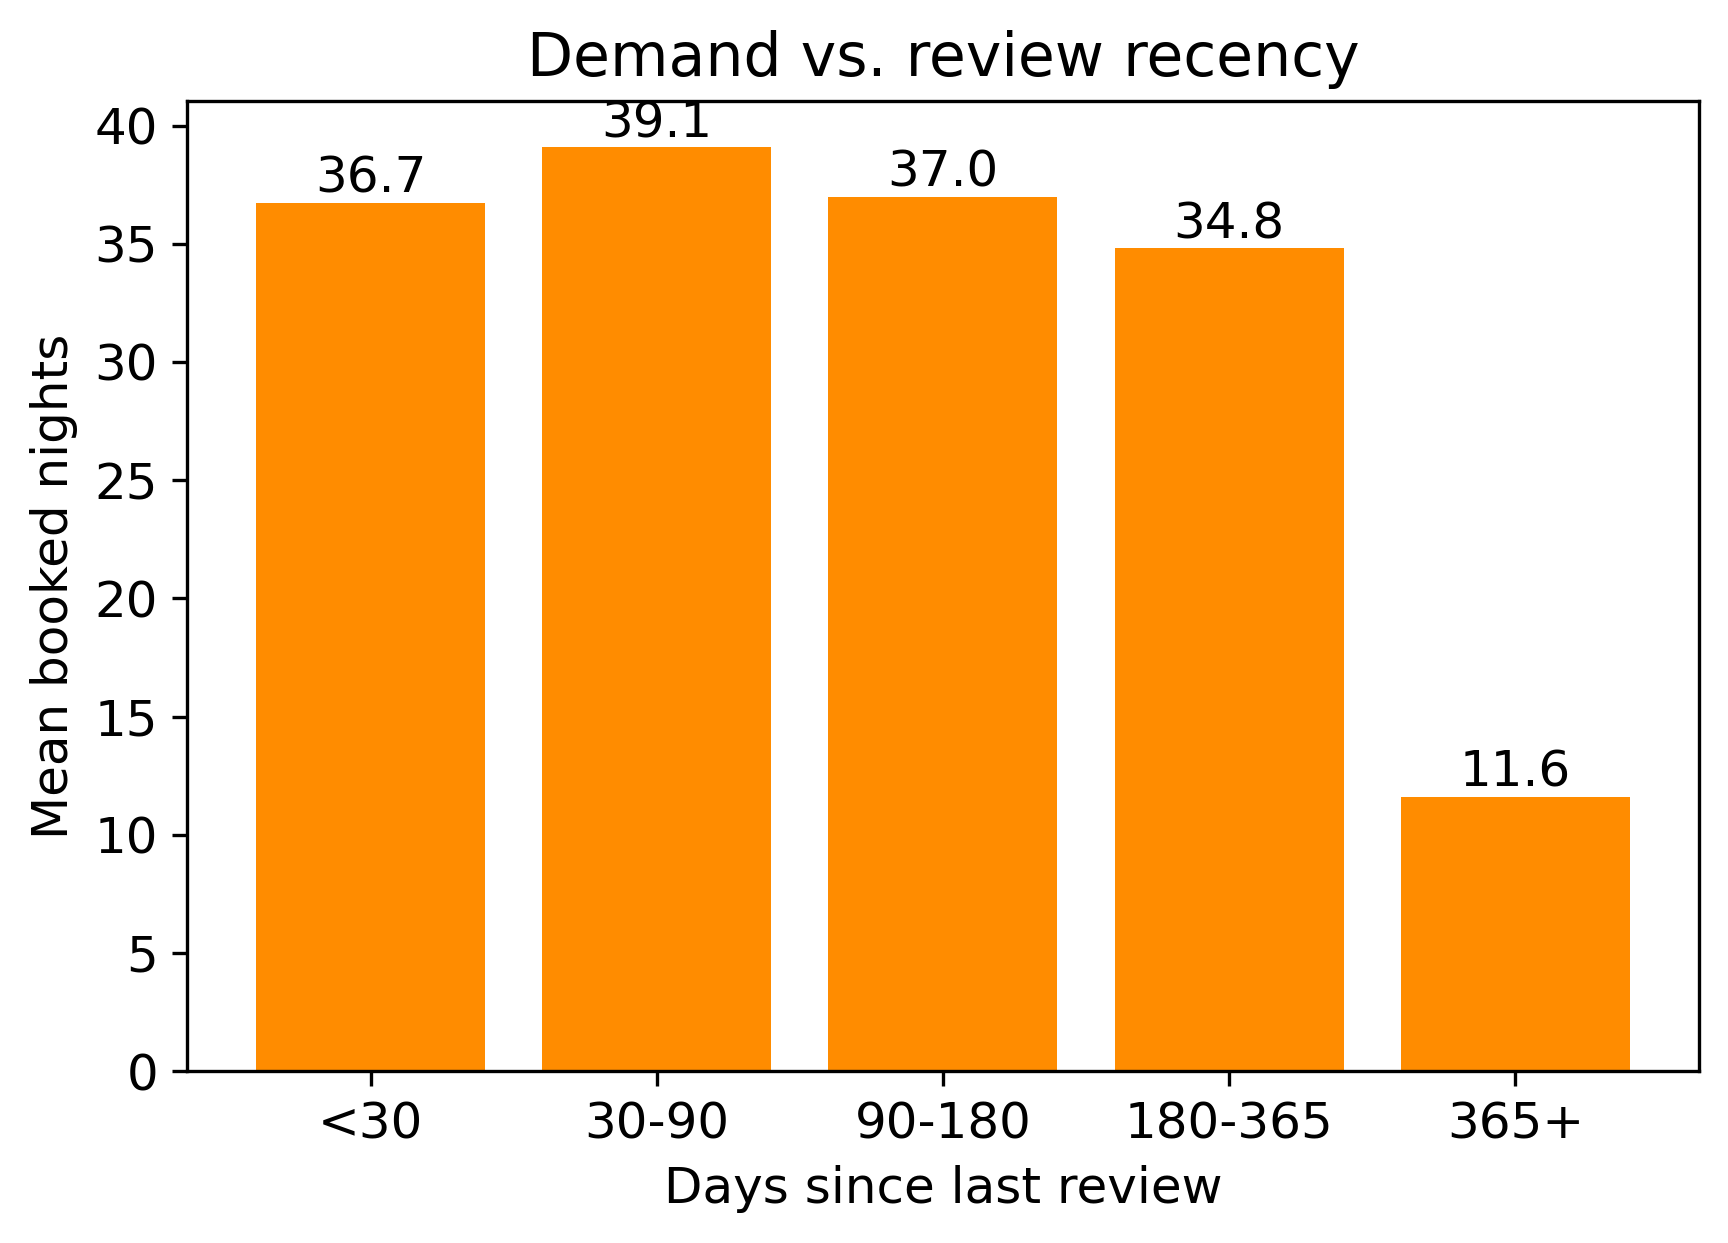
\includegraphics[width=\columnwidth]{fig10_review.png}
\caption{Mean target demand by review recency. Listings reviewed recently are
booked substantially more; those with year-old reviews are largely dormant.}
\label{fig:review}
\end{figure}

\subsection{Target construction by snapshot differencing}
Because no booking status exists, the demand target is reconstructed from how
availability evolves. Consider a target-quarter date $d$ observed across the
ordered snapshots that contain it. Let $a_{d}^{\text{first}}$ and
$a_{d}^{\text{last}}$ denote its availability at the earliest and latest snapshot
in which it appears, and let $n_d$ be the number of snapshots that observe it. The
date is counted as \emph{booked} when it was available at some point, is
unavailable at the last observation, and is seen at least twice:
\begin{equation}
b_d = \mathbb{1}\!\left[\,n_d \ge 2 \ \wedge\ \exists\,\text{available}\ \wedge\
a_{d}^{\text{last}}=\texttt{f}\,\right].
\label{eq:booked}
\end{equation}
The per-listing target is the sum over the quarter's dates,
$y=\sum_{d\in Q} b_d$, clipped to $[0,92]$. Requiring $n_d\ge 2$ and a genuine
available$\rightarrow$unavailable transition removes dates that were blocked from
the outset (host blocking) and dates observed only once, reducing noise relative
to a naive occupancy count. The two-observation requirement also guards against a
subtler artefact: listings that appear only once in the target-quarter window, such
as those listed very late, would otherwise contribute spurious zeros or ones that
reflect sampling rather than demand. By insisting that a booking be witnessed as a
transition across at least two snapshots, the construction ties every counted night
to observed evidence, which is what allows the recovered target to behave like a
genuine demand distribution rather than an artefact of the scraping cadence.

Empirically this construction produces exactly the demand-like shape expected of a
censored, zero-inflated count. For the February--April 2026 quarter the target has
mean $19.2$, median $2$, standard deviation $27.6$, and $47.7\%$ of listings at
zero (Fig.~\ref{fig:target}). By contrast, simply counting unavailable days yields
a left-skewed distribution with under $10\%$ zeros---dominated by host blocking
rather than demand---and is therefore not used.

\begin{figure}[!t]
\centering

\includegraphics[width=\columnwidth]{fig1_target_dist.png}
\caption{Target distribution (booked nights, Feb--Apr 2026, differencing
construction): sharply zero-inflated with a long right tail and a pile-up near the
upper bound.}
\label{fig:target}
\end{figure}

The contrast between the two candidate target definitions is stark and is what
justifies the differencing construction. Table~\ref{tab:targetdef} compares, on
the same listings and quarter, the naive occupancy count (number of unavailable
days) with the differencing target of \eqref{eq:booked}. The occupancy count is
\emph{left}-skewed with a median of $73$ of $92$ nights and fewer than $10\%$
zeros---most listings appear ``mostly unavailable'' simply because their hosts
have blocked the calendar---so it measures host behaviour, not demand. The
differencing target is \emph{right}-skewed, zero-inflated, and demand-like. Only
the latter is used henceforth.

\begin{table}[!t]
\caption{Naive occupancy count vs.\ the differencing target (same listings and
quarter). Only the differencing target is zero-inflated and demand-like.}
\label{tab:targetdef}
\centering
\small
\begin{tabular}{lccccc}
\toprule
Definition & mean & median & std & \%\,zero & skew \\
\midrule
Occupancy (unavailable days) & 57.4 & 73 & 32.5 & 8.0 & $-0.71$ \\
\textbf{Differencing (booked)} & 19.0 & 0 & 28.6 & 53.2 & $+1.32$ \\
\bottomrule
\end{tabular}
\end{table}

Table~\ref{tab:targetstats} reports the differencing-target statistics for each of
the three setups. All three are strongly zero-inflated (about half the listings at
zero) with comparable spread, confirming that the same difficult, censored
distribution is being modelled in every period.

\begin{table}[!t]
\caption{Differencing-target statistics by setup.}
\label{tab:targetstats}
\centering
\small
\begin{tabular}{lccccc}
\toprule
Setup (target quarter) & $n$ & mean & median & std & \%\,zero \\
\midrule
A (Q4 2025) & 36,111 & 21.9 & 2 & 29.6 & 46.9 \\
B (Q1 2026) & 36,282 & 16.3 & 1 & 25.0 & 48.7 \\
C (Feb--Apr 2026) & 36,282 & 19.2 & 2 & 27.7 & 47.7 \\
\bottomrule
\end{tabular}
\end{table}

\subsection{Prediction setups}
The problem is to predict, for each listing, the booked nights in a future quarter
from a behavioural history that ends before that quarter begins. Because the
snapshots span a fixed ten-month window, three leakage-safe setups are possible,
differing in the target quarter and the amount of prior history
(Table~\ref{tab:setups}). Setup~C, with a seven-month history predicting
February--April 2026, is the deepest-history configuration the data permit and is
used as the primary model; Setups~A and B provide temporal validation. For each setup, the population of
listings to be scored---the \emph{universe}---is fixed to those present in the
snapshot immediately preceding the target quarter, which is the natural set of
listings ``known'' at the moment a forecast would be issued. A listing that exists
in that snapshot but has no earlier behavioural history contributes a cold-start row
whose behavioural features are missing and are imputed; such rows are retained
rather than discarded, both because they are a genuine part of the operational
population and because their prevalence is itself informative about the market. This
choice keeps the evaluation honest: the model is asked to score exactly the set of
listings a platform would need to score in practice, including the difficult
newcomers.

\begin{table}[!t]
\caption{Prediction setups (history $\rightarrow$ target).}
\label{tab:setups}
\centering
\small
\begin{tabular}{llll}
\toprule
Setup & History window & Target quarter & Listings \\
\midrule
A & Q3 2025 (3 mo) & Q4 2025 & 36,111 \\
B & Q3+Q4 2025 (6 mo) & Q1 2026 & 36,282 \\
\textbf{C} & \textbf{Jul 2025--Jan 2026 (7 mo)} & \textbf{Feb--Apr 2026} & 36,282 \\
\bottomrule
\end{tabular}
\end{table}

\subsection{Metric and evaluation protocol}
Predictions are evaluated by Mean Squared Error,
\begin{equation}
\text{MSE}=\frac{1}{n}\sum_{i=1}^{n}\bigl(y_i-\hat y_i\bigr)^2,
\label{eq:mse}
\end{equation}
and the coefficient of determination $R^2$, which is scale-free and therefore the
primary basis for comparison. Two evaluation regimes are used. For model
development and blend-weight estimation, $5$-fold cross-validation is applied on a
development set. For an unbiased final estimate, listings are split once into an
$80\%$ development set and a $20\%$ held-out test set (fixed seed); models are
fitted on the development set and evaluated once on the untouched test set.
Reporting both regimes is deliberate: the cross-validation estimate is used for
model selection and for learning the blend weights, but because those weights are
themselves fitted to out-of-fold predictions, a cross-validation score can be
mildly optimistic. The disjoint held-out set, evaluated exactly once with no
tuning, provides the unbiased figure of merit, and the proximity of the two
numbers reported in Section~\ref{sec:results} is itself an experimental result: it
demonstrates that the cross-validation was honest and that the model does not
overfit the listings it was trained on. All splits are over listings rather than
over time within the history window, so a listing never appears in both training
and evaluation; the temporal separation between features and target is enforced
separately, by construction, through the leakage-safe feature definitions.

%==============================================================================
\section{Methodology}
\label{sec:method}

\subsection{Feature engineering}
Each listing is described by a flat feature vector assembled from its calendar
history and its most recent \texttt{listings} record. The engineered families are
summarised in Table~\ref{tab:featfam}. Behavioural features are computed per
sub-period (each quarter of the history window and the most recent month) and
include booked-night counts and rates, occupancy and availability rates,
availability churn (transition counts), and monthly booked-day series from which a
trend and a recency signal are derived. Property and host metadata come from the
snapshot immediately preceding the target quarter. Reviews contribute counts and a
recency signal. Geography is summarised by a $K$-Means cluster over
latitude/longitude in addition to the raw neighbourhood field, and short binary
keyword flags are extracted from the listing title. Crucially, forward-looking
availability fields (e.g.\ \texttt{availability\_30/60/90}) are \emph{excluded},
because in a pre-target snapshot they encode the host's intended availability for
the target quarter and would leak the label. This exclusion is deliberate and
non-trivial: the forward-looking availability counters are among the most
predictive fields in the raw data precisely because they encode the host's planned
availability for the very window being predicted, and retaining them would inflate
the reported accuracy while destroying the model's validity as a genuine forecast.
More broadly, every behavioural feature is computed only from calendar dates that
lie strictly before the target quarter, and the static attributes are taken from
the snapshot immediately preceding it, so no information about the target period
enters the feature matrix through any channel.

The behavioural families deserve emphasis because, as the importance and ablation
analyses later confirm, they carry almost all of the predictive signal. Occupancy
and booking rates summarise how intensively a listing was used in each recent
sub-period; churn counts (the number of availability transitions) distinguish an
actively managed listing from a static one; the monthly booked-day series captures
whether demand is accelerating or decaying heading into the target quarter; and the
recency block, computed over the most recent month, provides the single strongest
predictor by giving the model the freshest available evidence of activity.

\begin{table}[!t]
\caption{Engineered feature families.}
\label{tab:featfam}
\centering
\small
\begin{tabular}{lp{1.55in}}
\toprule
Family & Representative features \\
\midrule
Per-quarter behaviour & booked/occupancy/availability rate, churn \\
Monthly trajectory & booked days per month; trend; recency \\
Quarter-over-quarter & booking-rate change; half-year totals \\
Property/host metadata & type, capacity, bed/bath, host flags, reviews scores \\
Review velocity & counts in trailing windows; recency \\
Geographic & neighbourhood; $K$-Means cluster of (lat, lon) \\
Text keywords & luxury/private/cozy/\dots\ title flags \\
\bottomrule
\end{tabular}
\end{table}

Table~\ref{tab:featinv} gives an approximate breakdown of the engineered matrix by
family. The bulk of the columns are behavioural aggregates derived from the
calendar, computed separately for each historical quarter and for the most recent
month so that the model sees both the level and the trend of activity; the property
and host metadata contribute a smaller block of largely static attributes, and the
review, geographic, and text families are compact. This composition---behaviour
dominant, metadata secondary---mirrors the importance ranking reported later and is
a direct consequence of the fact that a listing's own recent booking behaviour is by
far the strongest available predictor of its near-future demand.

\begin{table}[!t]
\caption{Approximate composition of the engineered feature matrix by family.}
\label{tab:featinv}
\centering
\small
\begin{tabular}{lcp{1.25in}}
\toprule
Family & \# feats & Representative definition \\
\midrule
Per-quarter behaviour & $\sim$26 & booked/occupancy/availability rate; churn \\
Monthly trajectory & $\sim$9 & booked days per month; trend; recency \\
Quarter-over-quarter & $\sim$5 & booking-rate change; half-year totals \\
Property/host metadata & $\sim$25 & type, capacity, host flags, review scores \\
Review velocity & $\sim$5 & counts in windows; days since last review \\
Geographic & $\sim$3 & neighbourhood; K-Means cluster of (lat,lon) \\
Text keywords & $\sim$8 & binary title flags; title length \\
\bottomrule
\end{tabular}
\end{table}

\subsection{Preprocessing and the target encoder}
Every preprocessing step lives inside a column transformer that is fitted only on
the training fold, keeping the pipeline leakage-free. Numeric columns are
median-imputed; low-cardinality categoricals are one-hot encoded; and
high-cardinality location fields (neighbourhood) are handled by a $K$-fold target
encoder with additive smoothing. Writing $\mu$ for the global target mean and,
for a category level $c$ with $n_c$ rows and category mean $\bar y_c$, the
smoothed encoding is
\begin{equation}
e_c=\frac{n_c\,\bar y_c+\alpha\,\mu}{n_c+\alpha},\qquad \alpha=20,
\label{eq:te}
\end{equation}
so rare levels shrink toward $\mu$ and common levels approach $\bar y_c$. To
prevent a row from informing its own encoding, the encoder is fitted in an inner
$K$-fold loop: the value assigned to a training row in inner fold $\mathcal F_k$
uses statistics computed only on the complementary folds,
\begin{equation}
\tilde e_i=e^{\,(-\mathcal F_k)}_{\,x_i},\qquad i\in\mathcal F_k.
\label{eq:tekfold}
\end{equation}
Validation and test rows use the full-training map, and unseen levels fall back to
$\mu$. The multi-snapshot construction of \eqref{eq:booked} is central to
controlling label noise. A single snapshot cannot distinguish a booked date from a
host-blocked one, because both appear simply as \texttt{unavailable}. Observing the
same date across several snapshots, however, exposes its \emph{transition}: a date
that is offered (available) early and taken (unavailable) later is far more likely
to reflect a genuine booking than a date that is unavailable from the first moment
it is observed, which is almost certainly a host block. Requiring at least two
observations and a true available-to-unavailable transition therefore filters out
the dominant source of contamination, at the cost of missing bookings that were
already committed before the first snapshot or that occurred after the last. This
trade-off is the reason the differencing target, while still a proxy, is markedly
cleaner than the raw occupancy count, and it is the single most consequential
modelling decision in the study.

\subsection{Base learners}
Six heterogeneous learners span the linear, bagging, boosting, and neural-network
families: Linear Regression (a scaled interpretable baseline), Random Forest
\cite{breiman2001}, XGBoost \cite{chen2016xgboost}, LightGBM \cite{ke2017lightgbm},
CatBoost \cite{prokhorenkova2018catboost}, and a PyTorch \cite{paszke2019pytorch}
multi-layer perceptron trained with the Adam optimiser \cite{kingma2015adam}. The
MLP has three hidden layers ($256\!\to\!128\!\to\!64$) with batch normalisation,
ReLU, and dropout, and is trained directly on the raw (untransformed) target; a
$\log(1+y)$ transform, effective on the Kaggle-era formulation of this problem,
degraded its accuracy here. Adam updates each parameter using the standard moment
estimates $m_t=\beta_1 m_{t-1}+(1-\beta_1)g_t$ and
$v_t=\beta_2 v_{t-1}+(1-\beta_2)g_t^2$ of the gradient $g_t$. XGBoost's regularised
learning objective makes its complexity penalty explicit:
\begin{equation}
\mathcal{L}(\phi) = \sum_{i=1}^{n}\ell(y_i,\hat y_i) + \sum_{k=1}^{K}\Omega(f_k),
\label{eq:xgb-obj}
\end{equation}
where $K$ is the number of trees in the ensemble and
$\Omega(f_k)=\gamma T_k+\tfrac12\lambda\lVert w_k\rVert^2$ penalises each tree's
leaf count $T_k$ and leaf-weight norm, discouraging overly complex trees; $\lambda$
is tuned (Section~\ref{sec:hpsearch}) and fixed at $\lambda=3$ for the default model.
All are trained on the same preprocessed matrix
with squared-error loss; the tree models exploit the encoded categorical splits,
while the linear baseline additionally uses feature scaling. Predictions are
clipped to $[0,92]$, both because the competition-style metric is defined on that
support and because no listing can be booked for more nights than the quarter
contains; clipping costs almost nothing in accuracy, as the vast majority of raw
predictions already fall inside the interval, but it removes the occasional
nonsensical value that a linear model in particular can produce at the extremes. No
learner is given access to the target of any other listing, and the same fixed
random seed governs every model so that the comparison among them, and the estimated
blend weights, are exactly reproducible.

\subsection{Convex weighted blend}
Rather than selecting a single learner, the out-of-fold predictions of the $m=6$
learners are stacked into a matrix $\mathbf P\in\mathbb R^{n\times m}$ and combined
by a convex weighted average. The weights minimise the blended MSE subject to a
probability-simplex constraint:
\begin{align}
\min_{\mathbf w\in\mathbb R^{m}}\quad
&\frac{1}{n}\sum_{i=1}^{n}\!\Bigl(y_i-\mathrm{clip}\bigl[(\mathbf P\mathbf w)_i,0,92\bigr]\Bigr)^2
\label{eq:blend}\\
\text{s.t.}\quad &\textstyle\sum_{j=1}^{m}w_j=1,\qquad 0\le w_j\le 1.
\label{eq:blendc}
\end{align}
The equality and box constraints keep the blend on the same scale as its inputs
and prevent any single learner from receiving a runaway weight. Problem
\eqref{eq:blend}--\eqref{eq:blendc} is solved by Sequential Least-Squares
Quadratic Programming (SLSQP) from the uniform start $w_j^{(0)}=1/m$; negligible
weights ($w_j<10^{-4}$) are then zeroed and the remainder renormalised. The same
weights, learned on development out-of-fold predictions, are applied to the
held-out test predictions.

\subsection{Two-stage hurdle model (evaluated as an ablation)}
Given the large zero mass, a natural alternative is a two-part hurdle model that
factorises the prediction into a Bernoulli hurdle and a positive-count expert,
\begin{equation}
\mathbb E[y\mid\mathbf x]=\underbrace{\Pr(y>0\mid\mathbf x)}_{\text{classifier }p(\mathbf x)}
\cdot
\underbrace{\mathbb E[y\mid y>0,\mathbf x]}_{\text{regressor }r(\mathbf x)},
\label{eq:hurdle}
\end{equation}
where the classifier is trained on the binary label $\mathbb 1[y>0]$ over all rows
and the regressor is fitted only on booked listings. The expected-value prediction
$\hat y=\mathrm{clip}(p(\mathbf x)\,r(\mathbf x),0,92)$ is evaluated in
Section~\ref{sec:ablation}. The appeal of this formulation is that it separates the
two decisions that the zero-inflated target conflates: a classifier can specialise
in recognising the large dormant population, for which the answer is a
near-deterministic zero, while a separate regressor, trained only on booked
listings, can focus on the shape of the positive counts without being pulled toward
zero by the mass of inactive listings. A hard-gated variant, which outputs zero
whenever the classifier's probability falls below a threshold, was also evaluated;
it degrades the squared-error metric because the metric rewards the expected value
rather than a thresholded decision, so only the expected-value combination is
retained for comparison. The empirical outcome---that neither variant improves on
the direct blend---is reported and discussed in Section~\ref{sec:ablation}.

\subsection{Hyper-parameter search}
\label{sec:hpsearch}
The two boosted-tree learners most likely to benefit from tuning, XGBoost and
LightGBM, were tuned by a randomized search of $30$ configurations per family
under the same $5$-fold cross-validation, sampling the learning rate and
regularisation terms log-uniformly and the tree-shape parameters over sensible
integer ranges. To keep the search efficient, the leakage-safe preprocessing was
computed once per fold and cached, so each configuration re-fits only the model.
As reported in Section~\ref{sec:ablation}, the tuned learners did not
meaningfully improve on their defaults and the tuned blend did not exceed the
default blend, indicating that the models operate near their capacity for this
feature set and that the residual error is data-limited rather than
capacity-limited. Default settings are therefore retained for the primary model in
the interest of simplicity and reproducibility.

\subsection{Computational cost}
The pipeline is inexpensive. Building the feature matrix from the multi-million-row
calendars is a one-time aggregation that dominates wall-clock time but is trivially
parallel over listings. Each learner fits in seconds to a few minutes on a
$36{,}000$-row matrix on a single multi-core CPU; the SLSQP blend optimises only
$m=6$ weights over a cached matrix of out-of-fold predictions and converges in well
under a second. Because the out-of-fold predictions are cached, the blend and every
post-hoc diagnostic can be recomputed without retraining, which makes the entire
ablation study cheap to run.

\subsection{Reproducibility}
All results use a single fixed seed governing the development/test split, the
cross-validation partitions, and the inner target-encoding folds. The
implementation is in Python with scikit-learn (preprocessing, linear and
random-forest models, cross-validation), XGBoost, LightGBM, CatBoost, PyTorch
(the MLP sixth learner), and
\texttt{scipy.optimize} for the SLSQP blend. Out-of-fold predictions are cached so
that the blend and all diagnostics can be recomputed without retraining. The
software stack comprises Python~3.13 with scikit-learn (preprocessing, the linear
and random-forest models, and cross-validation), XGBoost, LightGBM, and CatBoost
for the boosted learners, PyTorch~2.12 for the MLP, and \texttt{scipy.optimize} for
the SLSQP blend; all experiments run on a MacBook Air (Apple M4, 10-core CPU, 16GB
RAM, 512GB SSD) with no discrete GPU. The code is organised as a
sequence of stages---exploratory analysis, feature construction, one module per
model family, the blend, and the diagnostics---each of which reads and writes
intermediate artefacts to disk, so that any stage can be re-executed independently
and the full study reproduced end to end from the raw snapshots and a single seed.

%==============================================================================
\section{Results}
\label{sec:results}

\subsection{Main model and held-out performance}
Table~\ref{tab:heldout} reports the primary result: the performance of every
learner and of the blend on the $20\%$ held-out test set, alongside the
development cross-validation estimate, for Setup~C. The blend is the best
configuration on both partitions, reaching a held-out test $R^2$ of $0.654$
(MSE $260.9$). Figure~\ref{fig:modelcmp} visualises the held-out ranking.
Critically, the held-out $R^2$ ($0.654$) is within $0.011$ of the development
cross-validation estimate ($0.665$): the model does not overfit, and the
cross-validation figures reported elsewhere in the paper are honest rather than
optimistic. It is worth translating this accuracy into operational terms. An $R^2$
of about $0.65$ on a target with a standard deviation near $28$ nights corresponds
to a typical error on the order of ten nights per listing per quarter, concentrated
---as the residual analysis shows---on the ambiguous middle and the busiest
listings rather than on the large, easily identified dormant population. For the
ranking and resource-allocation applications that motivate the work, in which the
relative ordering of listings by expected demand matters more than the exact count,
this is a useful signal; for exact per-listing revenue projection it is a coarse
one, and the paper is careful not to overstate it. The value of the held-out
protocol is precisely that it lets a practitioner calibrate such expectations
against an unbiased estimate.

\begin{table}[!t]
\caption{Held-out performance (Setup~C; development $n=29{,}025$, held-out test
$n=7{,}257$). The blend is best on both partitions and generalises with a
negligible dev--test gap.}
\label{tab:heldout}
\centering
\begin{tabular}{lccc}
\toprule
Model & Dev $R^2$ & Test $R^2$ & Test MSE \\
\midrule
Linear Regression & 0.581 & 0.568 & 326.0 \\
MLP & 0.632 & 0.626 & 282.4 \\
CatBoost & 0.654 & 0.641 & 270.8 \\
Random Forest & 0.652 & 0.644 & 268.7 \\
XGBoost & 0.661 & 0.647 & 266.2 \\
LightGBM & 0.659 & 0.649 & 264.6 \\
\textbf{SLSQP blend} & \textbf{0.665} & \textbf{0.654} & \textbf{260.9} \\
\bottomrule
\end{tabular}
\end{table}

\begin{figure}[!t]
\centering
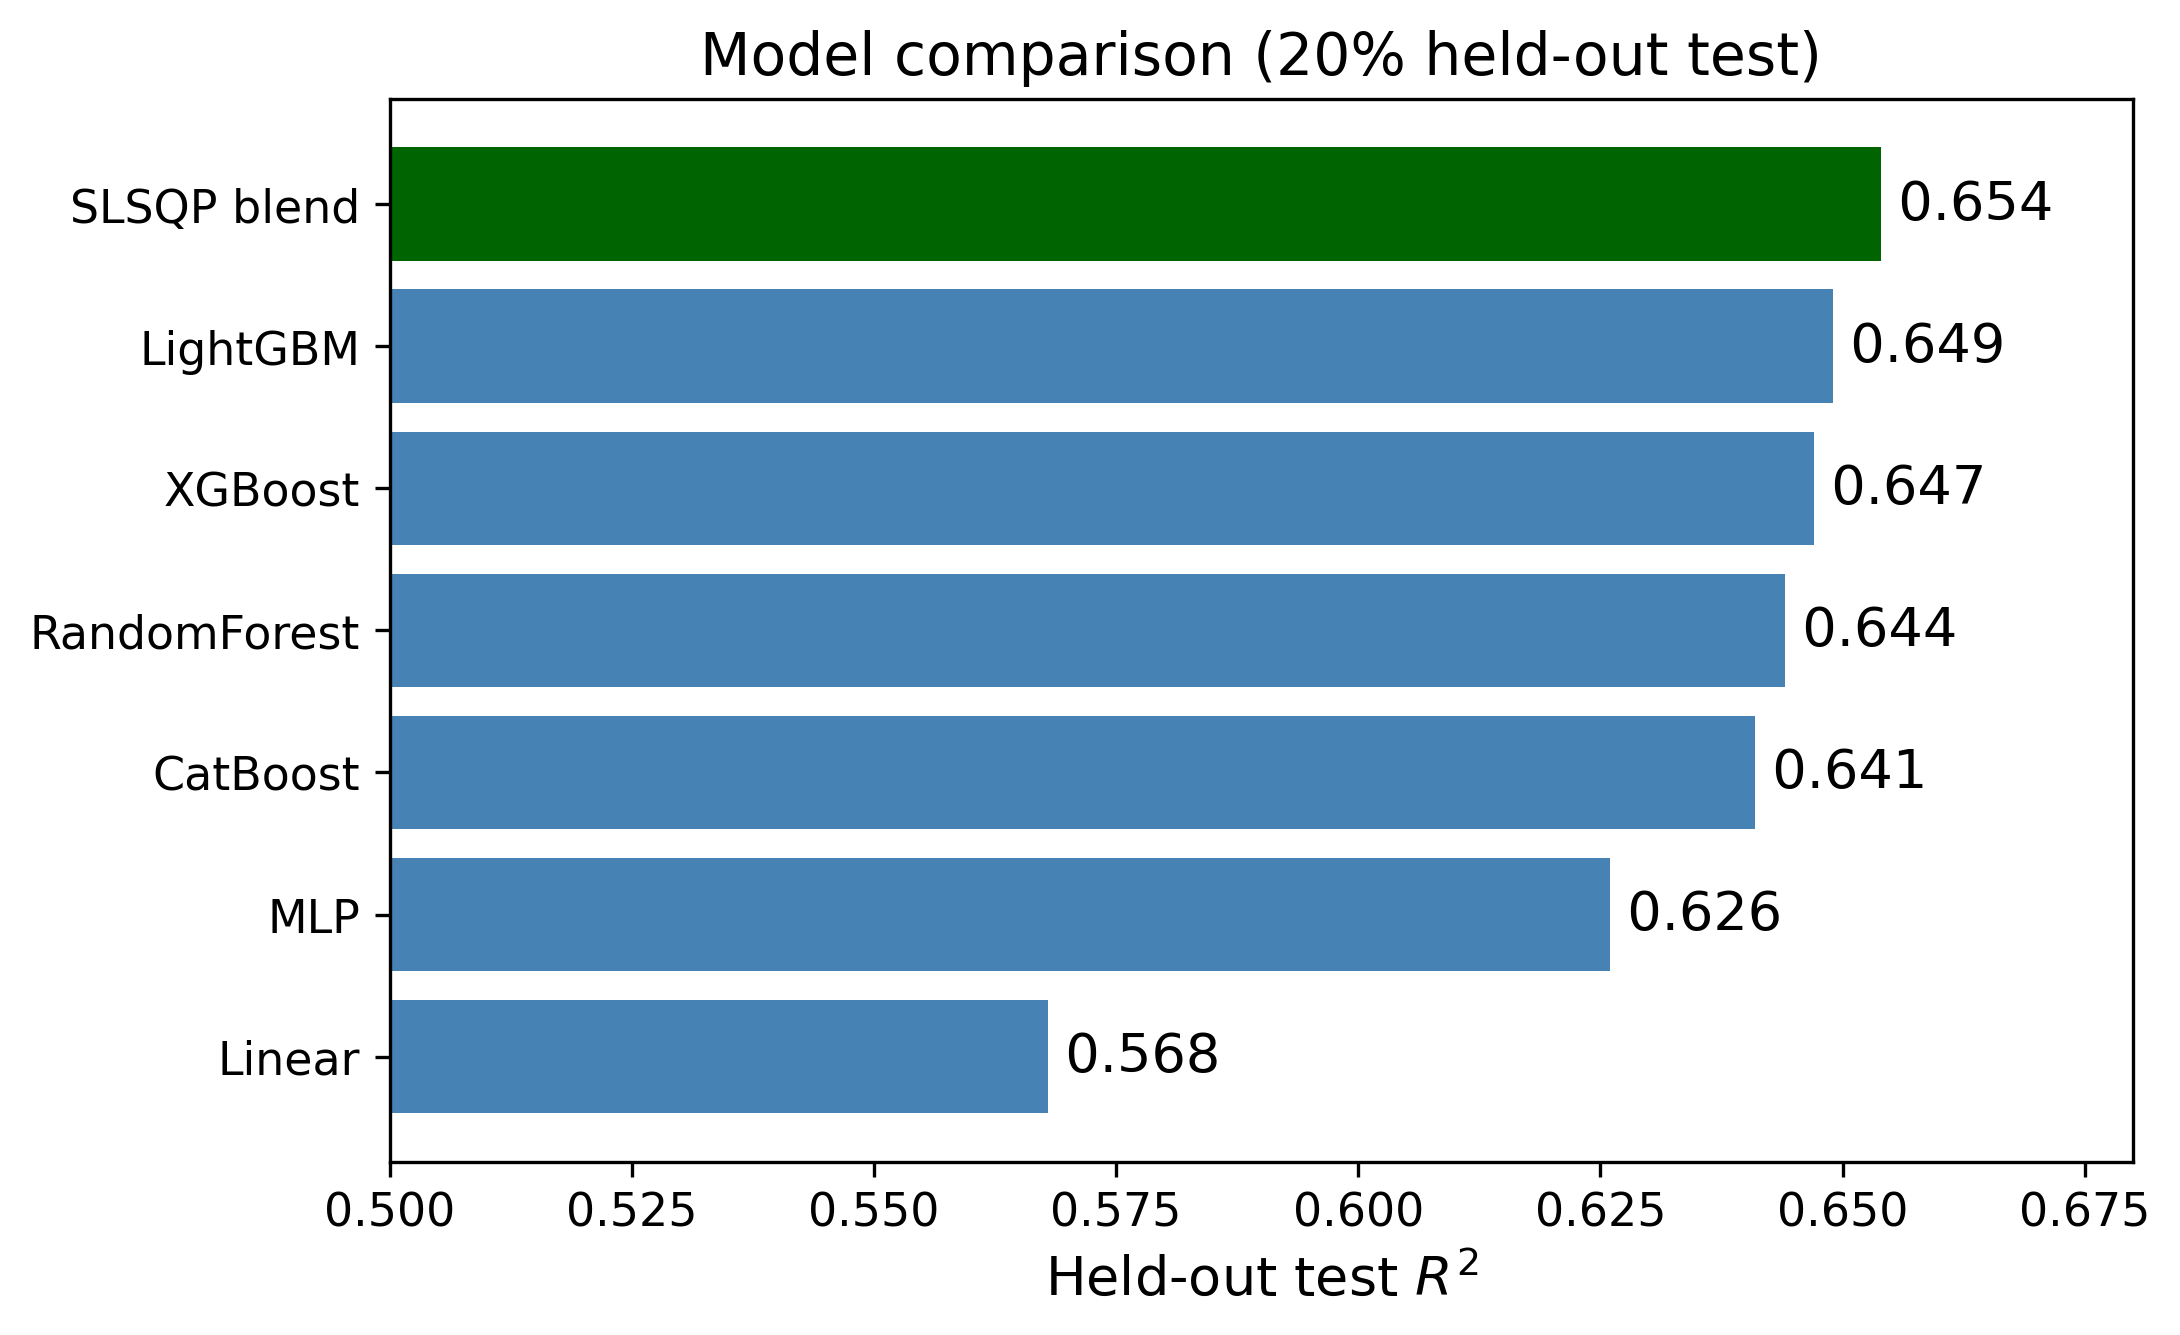
\includegraphics[width=\columnwidth]{fig4_model_compare.png}
\caption{Held-out test $R^2$ by model. The convex blend (green) improves on every
single learner.}
\label{fig:modelcmp}
\end{figure}

\subsection{Development comparison and model complementarity}
Table~\ref{tab:devcv} reports the full development-set cross-validation metrics for
Setup~C. The three gradient-boosting learners are close (LightGBM and XGBoost
lead among singles at $R^2=0.659$), Random Forest is competitive, and the linear
baseline trails, as expected on a non-linear, interaction-rich target. The blend
improves on every single learner in MSE, MAE, and $R^2$ simultaneously. The convex
weights concentrate on the complementary learners---Random Forest $0.37$, LightGBM
$0.34$, XGBoost $0.12$, the MLP $0.17$, CatBoost $0.00$, Linear $0.00$---rather than placing all
weight on the single best model, which is precisely why the blend improves: its
members make partially different errors, and the constrained optimisation exploits
that de-correlation. A naive equal-weight average, by contrast, is worse than the
best single model, because it lets the weaker learners drag the mean down; the
convex weighting is what converts the ensemble into a net gain.

\begin{table}[!t]
\caption{Development-set 5-fold CV (Setup~C, $n=36{,}282$).}
\label{tab:devcv}
\centering
\begin{tabular}{lccc}
\toprule
Model & MSE & MAE & $R^2$ \\
\midrule
Linear Regression & 322.7 & 11.88 & 0.578 \\
MLP & 279.0 & 10.11 & 0.635 \\
CatBoost & 266.3 & 9.98 & 0.652 \\
Random Forest & 263.0 & 9.73 & 0.656 \\
XGBoost & 260.9 & 9.75 & 0.659 \\
LightGBM & 260.8 & 9.70 & 0.659 \\
\textbf{SLSQP blend} & \textbf{256.1} & \textbf{9.67} & \textbf{0.665} \\
\bottomrule
\end{tabular}
\end{table}

\subsection{Temporal robustness}
To confirm that the method is not tuned to a single window, the identical pipeline
was applied to the three setups of Table~\ref{tab:setups}.
Table~\ref{tab:temporal} and Fig.~\ref{fig:temporal} report the blend performance,
now with the MLP included as a sixth learner in all three setups.
Accuracy is stable across all three independent target quarters, and the
seven-month history of Setup~C yields the strongest result, confirming that deeper
behavioural history helps. The stability across periods is meaningful because the
three quarters differ not only in calendar position but in seasonal demand and in
the amount of available history, yet the same pipeline, with no per-period
retuning, produces comparable accuracy in every case; this is direct evidence
against the concern that a single reported score might reflect a fortunate choice
of window. The intermediate dip at Setup~B is consistent with its winter target
quarter being both lower in demand and predicted from a shorter six-month history;
when the history is extended to seven months and the target shifts to the
February--April window, accuracy recovers and surpasses the other two settings.

\begin{table}[!t]
\caption{Cross-period robustness of the blend (5-fold CV).}
\label{tab:temporal}
\centering
\begin{tabular}{lcc}
\toprule
Setup & Target quarter & Blend $R^2$ \\
\midrule
A & Q4 2025 & 0.645 \\
B & Q1 2026 & 0.575 \\
\textbf{C} & \textbf{Feb--Apr 2026} & \textbf{0.665} \\
\bottomrule
\end{tabular}
\end{table}

\begin{figure}[!t]
\centering
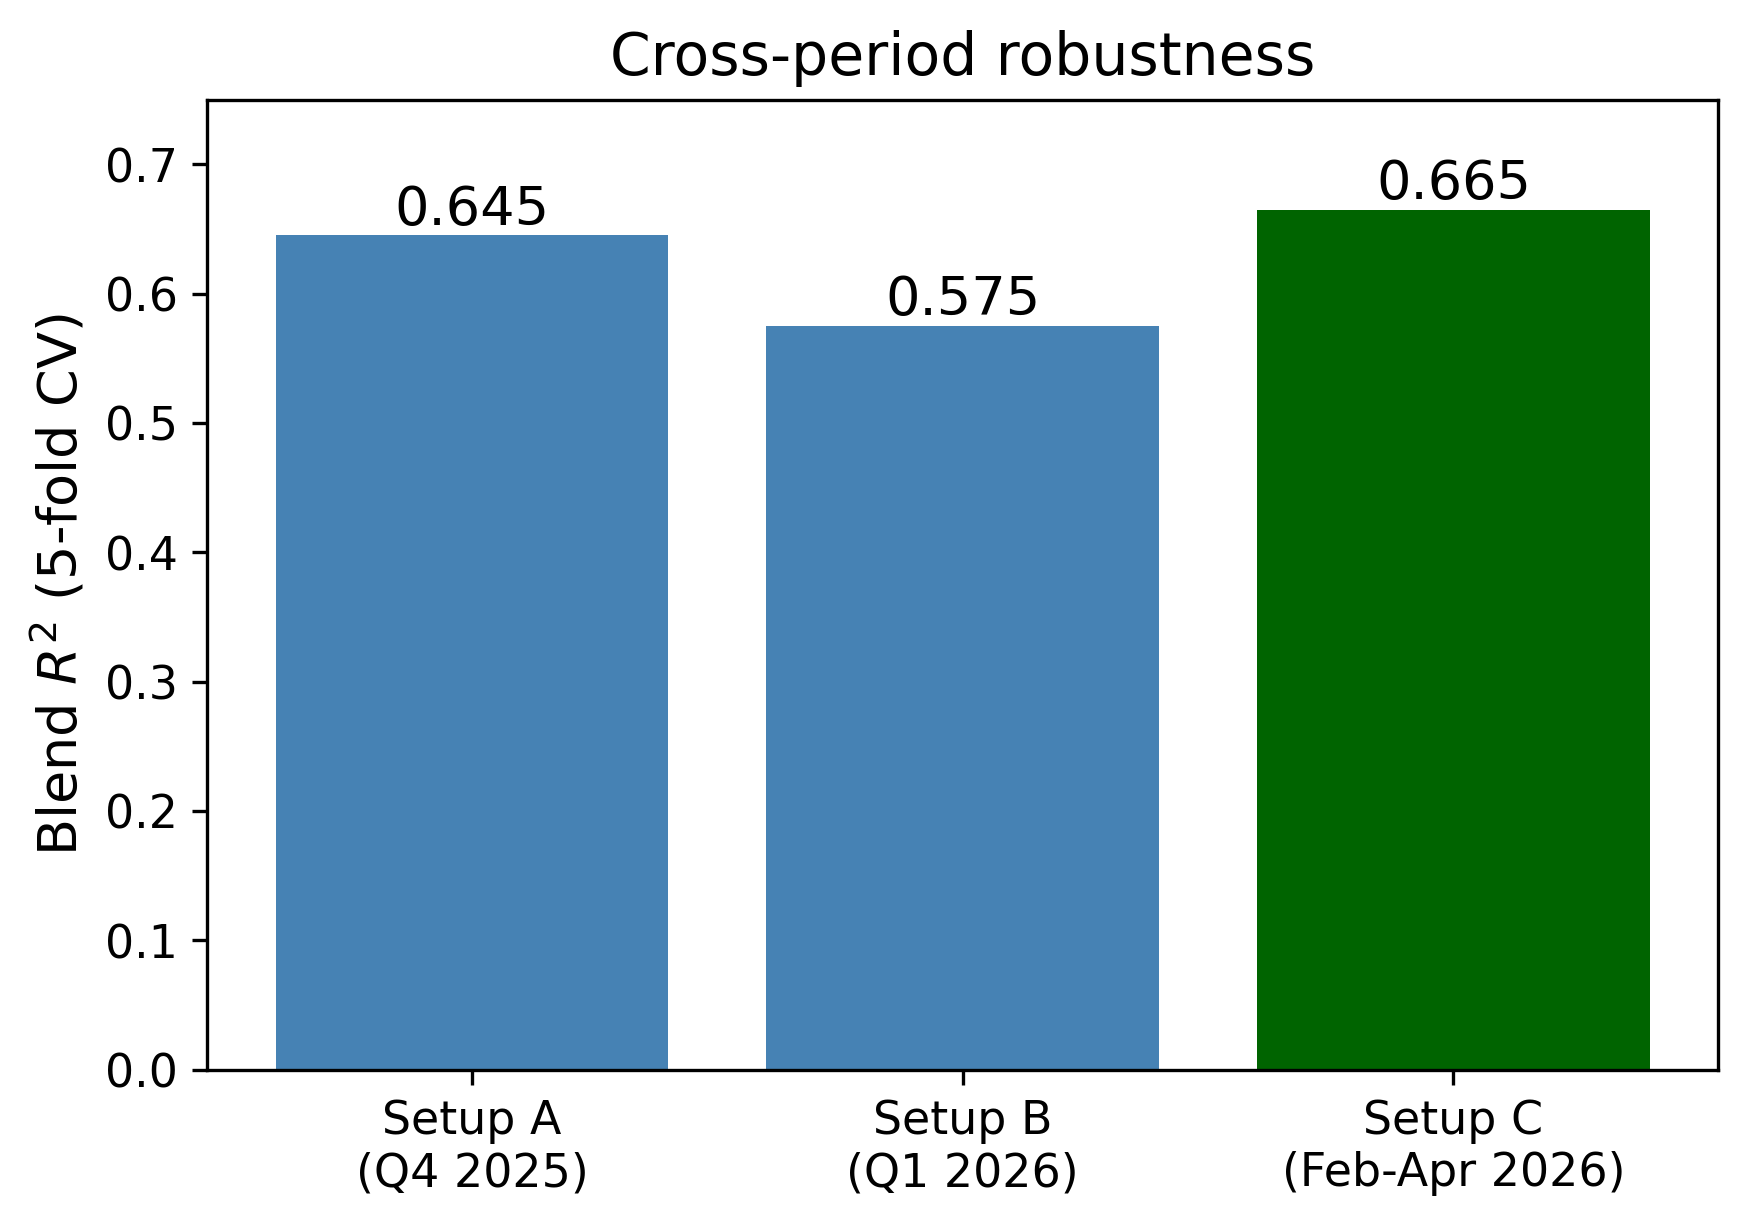
\includegraphics[width=\columnwidth]{fig5_temporal.png}
\caption{Blend $R^2$ across three independent target quarters. Performance is
stable, and the deepest-history setup (C) is strongest.}
\label{fig:temporal}
\end{figure}

\subsection{Statistical significance}
The blend's improvement over the best single learner is statistically significant.
On a paired test of per-listing squared errors, Setup~A gives $t=7.69$,
$p=1.6\times10^{-14}$ and Setup~B gives $t=5.99$, $p=2.1\times10^{-9}$; in both
cases the $95\%$ confidence interval on the mean squared-error reduction excludes
zero, and the non-parametric Wilcoxon signed-rank test agrees. The gain is small
in effect size, as expected---the blend only changes the minority of listings on
which the base learners disagree---but it is consistent and obtained at no extra
training cost, since the learners are already trained. The interpretation of the
effect size warrants care: a small $d_z$ does not mean the blend is unimportant,
but rather that its benefit is concentrated on the subset of listings where the
base learners genuinely disagree. On the large majority of listings---those that
are clearly dormant or clearly active---all learners already agree, and the blend
leaves them unchanged; the improvement accrues on the harder, ambiguous middle of
the distribution, which is precisely where a demand forecast is most valuable and
most difficult. The consistency of the effect across two independent quarters, each
with tens of thousands of paired observations, is what makes the improvement
trustworthy despite its modest per-listing magnitude.

\subsection{Residual analysis on the boundaries}
Because the target is bounded and zero-inflated, aggregate error can hide
systematic behaviour at the edges. Figure~\ref{fig:resid} shows standard residual
diagnostics for the blend. The residual-versus-fitted panel reveals clear
heteroscedasticity---errors widen as the predicted count grows---and the
residual-versus-true panel and the Q--Q plot confirm non-Gaussian, right-skewed
residuals with structure at both boundaries. Figure~\ref{fig:residbin} localises
the bias by binning listings by their true value: the model \emph{over-predicts}
the dormant and lightly-booked listings and \emph{under-predicts} the busiest ones,
the classic regression-to-the-mean behaviour of a least-squares estimator on a
censored target. Clipping removes impossible predictions but not this boundary
bias, which motivates the hurdle experiment reported next and the two-stage
extension discussed in Section~\ref{sec:limits}.

\begin{figure*}[!t]
\centering
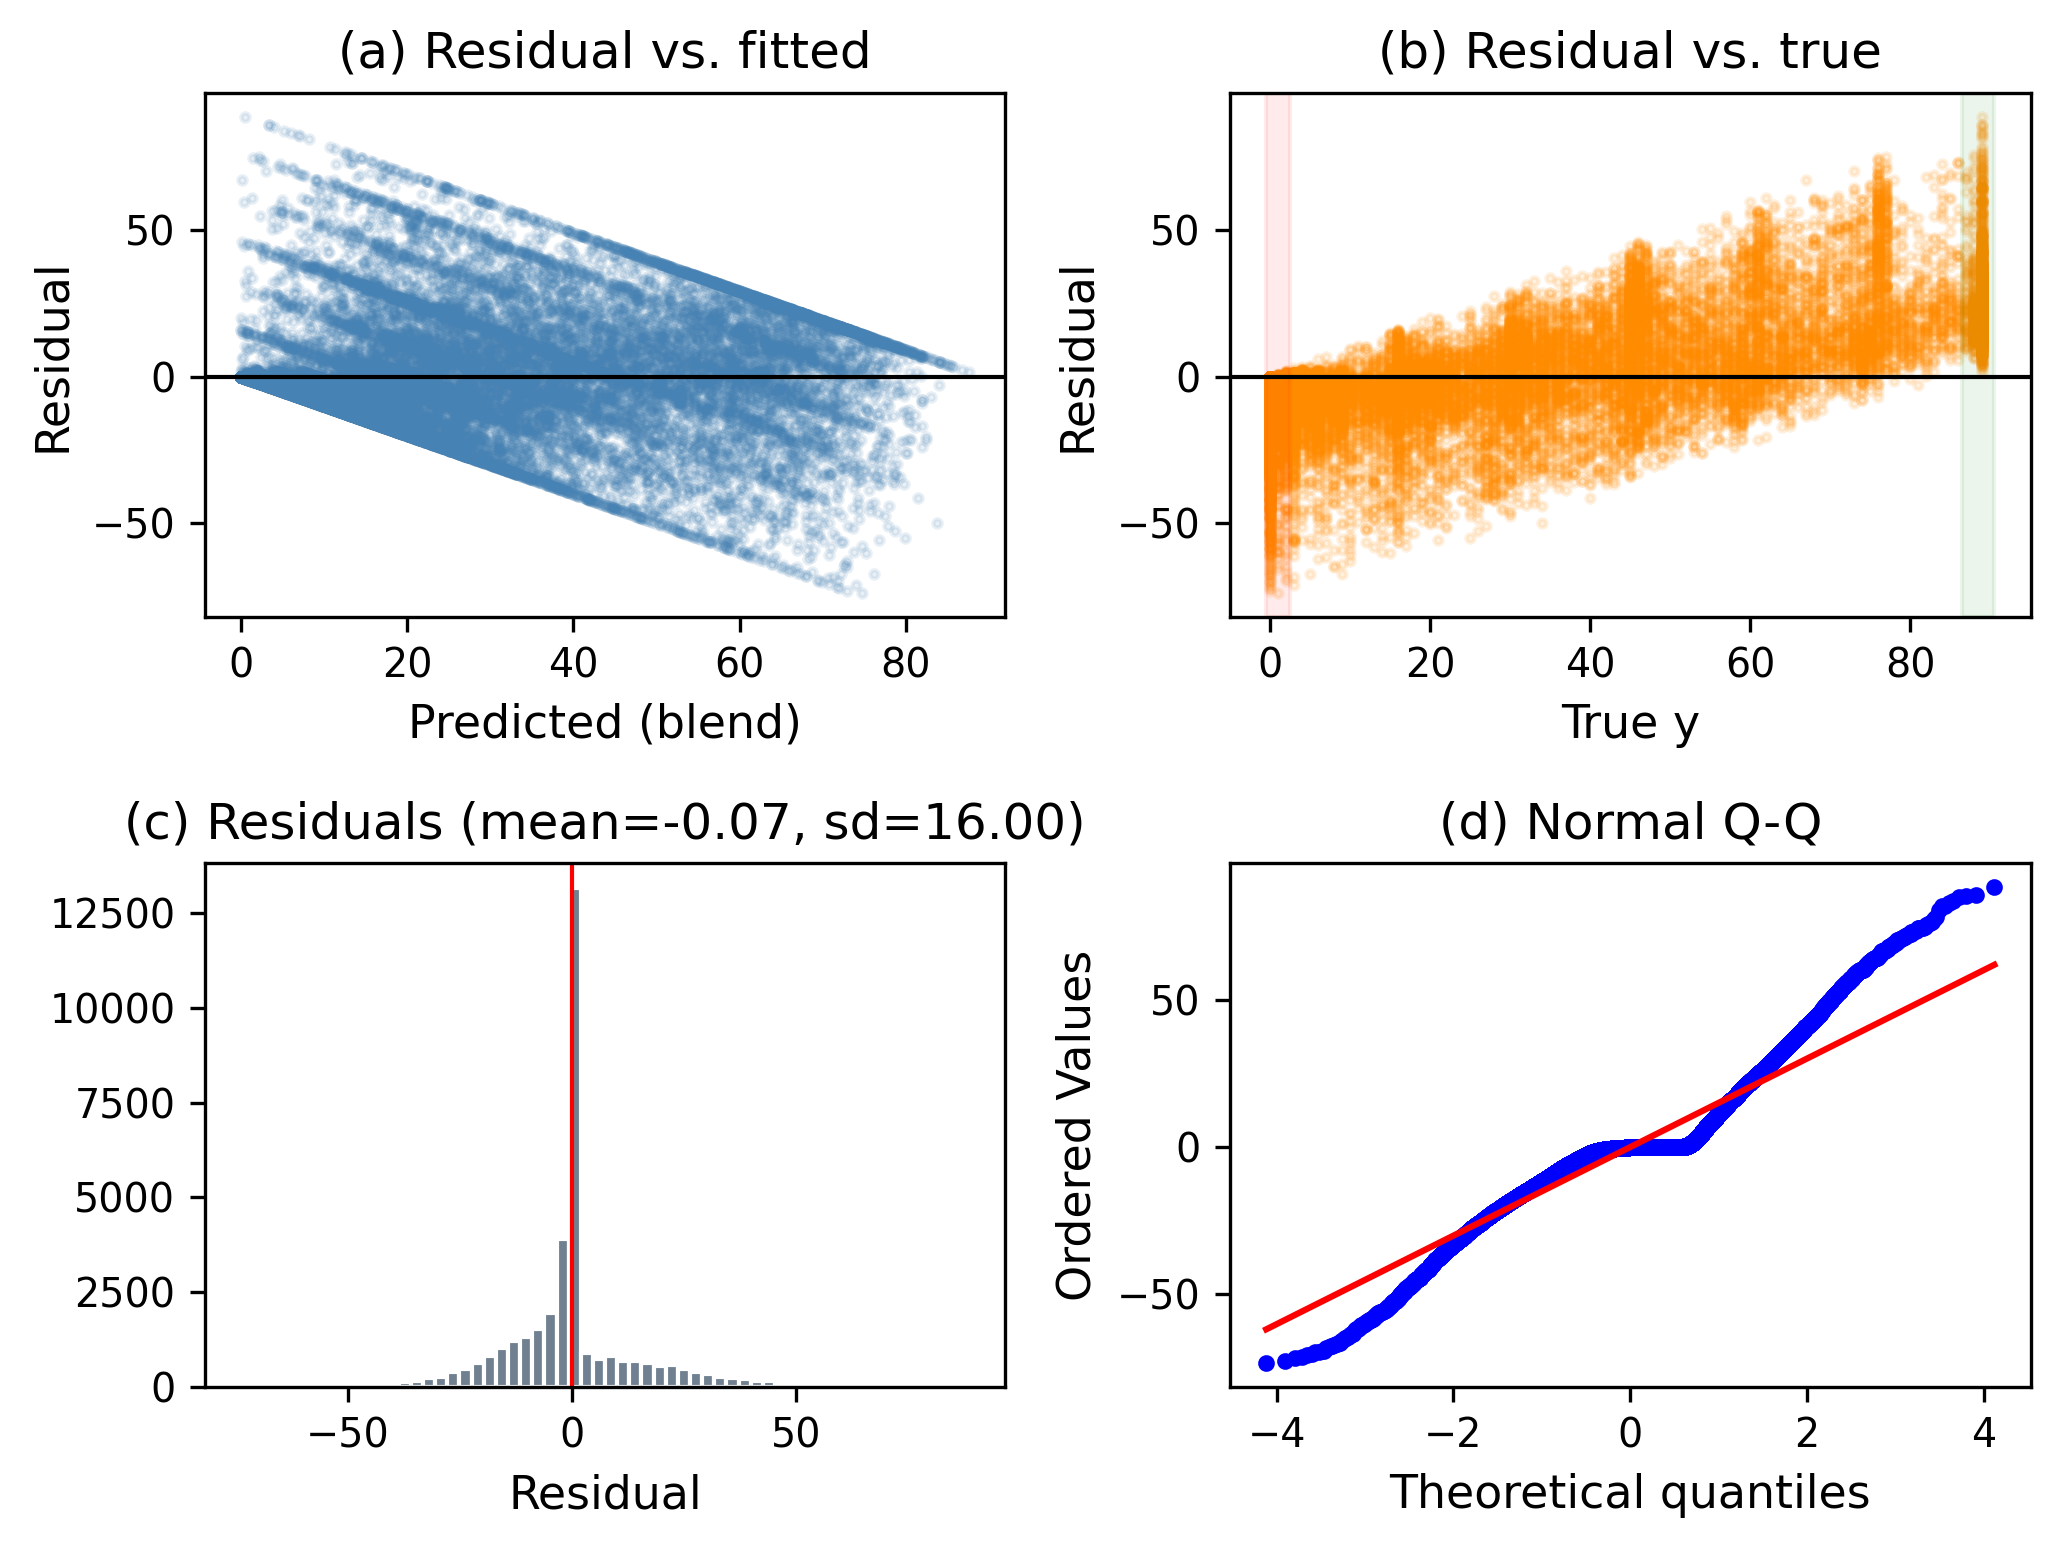
\includegraphics[width=0.96\textwidth]{fig7_residuals.png}
\caption{Residual diagnostics for the blend: (a) residual vs.\ fitted, (b)
residual vs.\ true with boundary bands, (c) residual histogram, (d) normal Q--Q.}
\label{fig:resid}
\end{figure*}

\begin{figure}[!t]
\centering
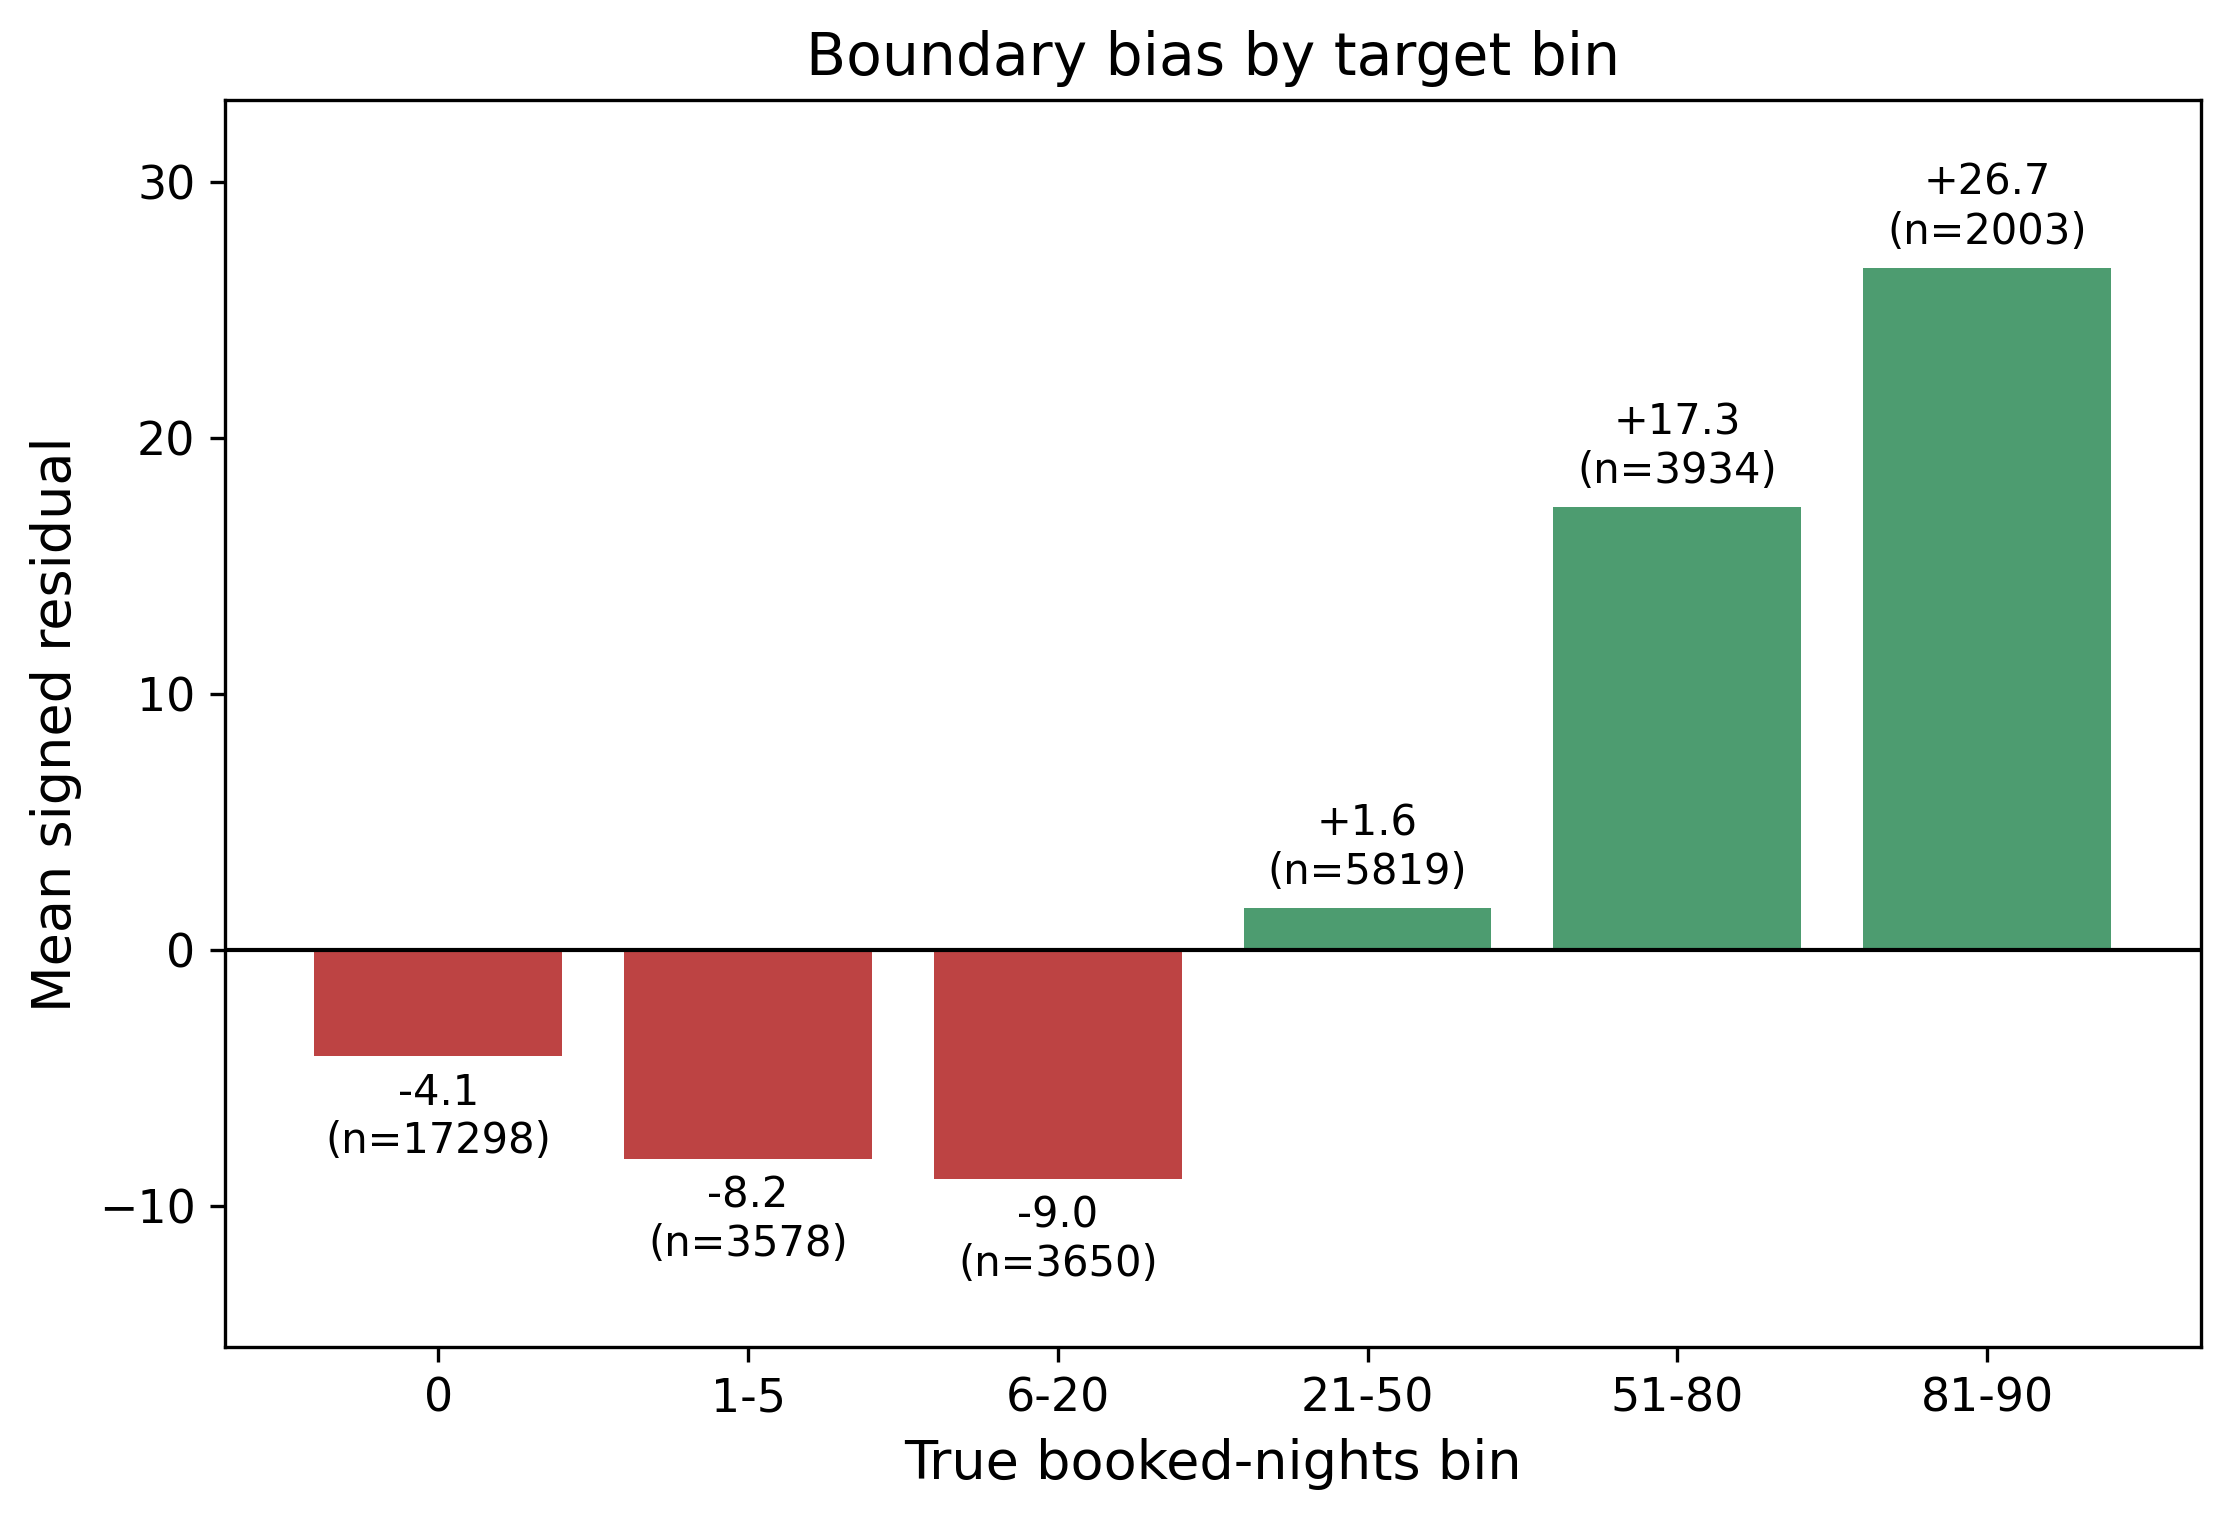
\includegraphics[width=\columnwidth]{fig8_residual_bins.png}
\caption{Mean signed residual by true-value bin. The model over-predicts the
low/zero range (red) and under-predicts the high range (green).}
\label{fig:residbin}
\end{figure}

\subsection{Feature importance}
Figure~\ref{fig:imp} shows the gain-based feature importances of the XGBoost
learner. The ranking is dominated by \emph{recent behavioural} signals: the most
recent month's booking rate and booked count (from January 2026, immediately
before the target quarter), a recency-weighted booking-rate feature, the
platform's own trailing occupancy estimate, the
seven-month booked total, and review recency. Static property and host metadata,
text keywords, and geography play only a supporting role. This confirms the
narrative of the residual and ablation analyses: demand is driven overwhelmingly
by a listing's own recent activity, which is why deeper and more recent history is
the feature-side lever that matters and why additional engineered families are
redundant once this signal is present.

\begin{figure*}[!t]
\centering
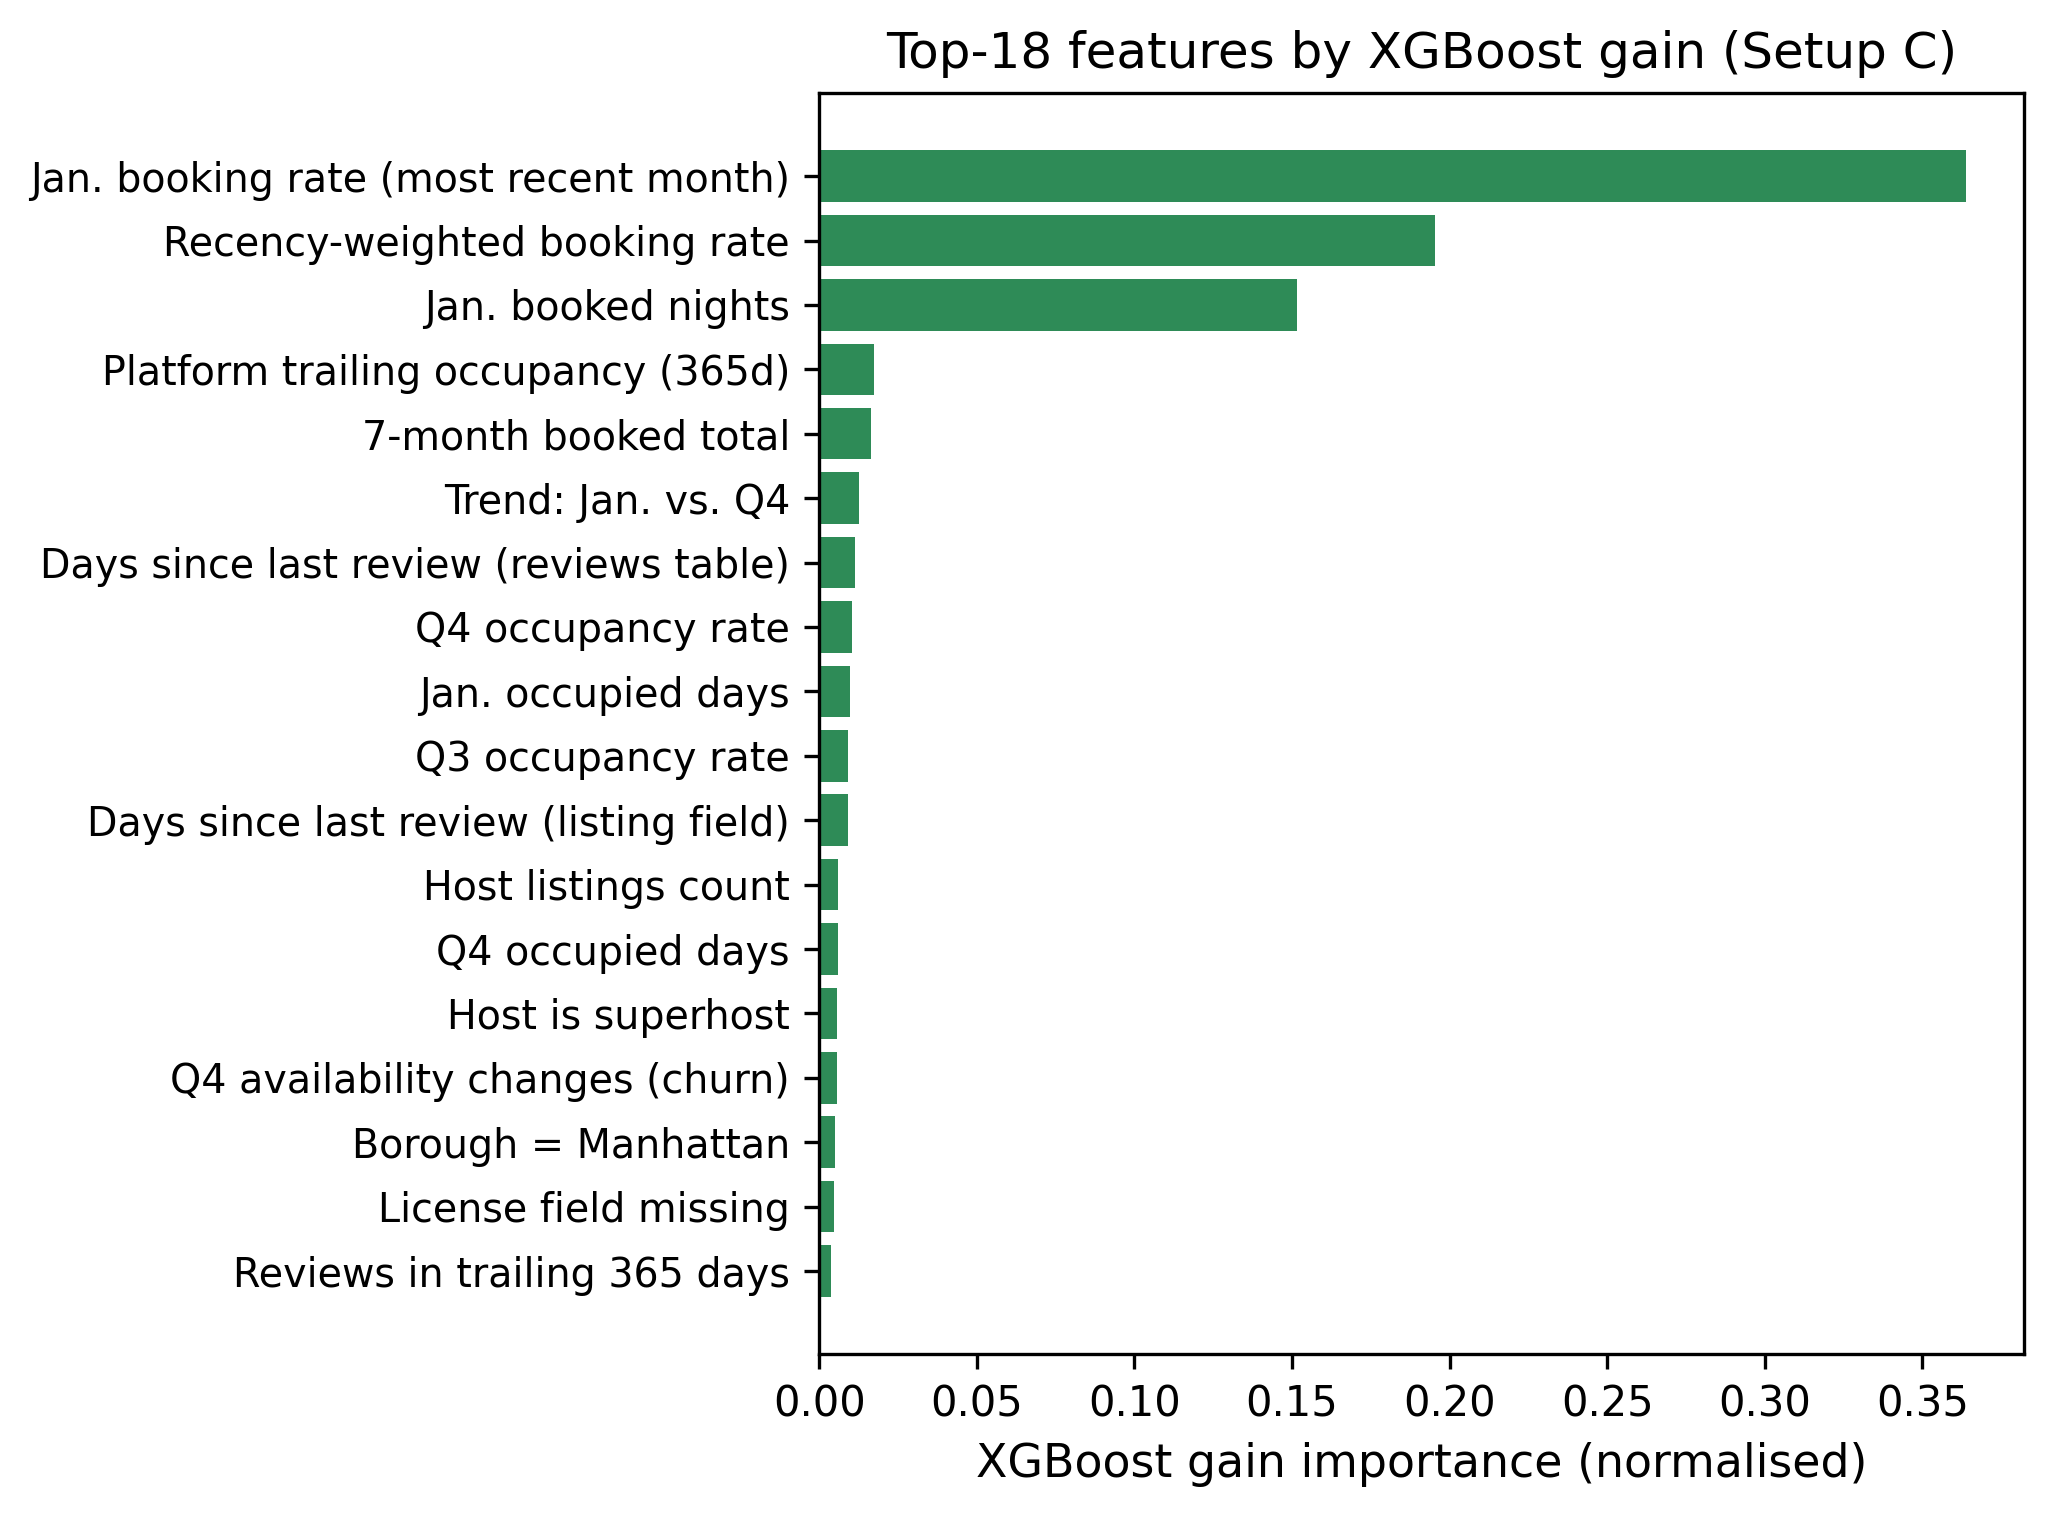
\includegraphics[width=0.96\textwidth]{fig9_importance.png}
\caption{XGBoost gain importances (Setup~C). Recent behavioural features---the
latest month's booking rate and count, a recency-weighted booking rate, trailing
occupancy, and review recency---dominate; static metadata is secondary.}
\label{fig:imp}
\end{figure*}

\subsection{Failure-case analysis}
A sample-level inspection of the largest errors complements the aggregate metrics.
Table~\ref{tab:failure} lists the development-set listings with the largest blend
residuals. Every one is a listing that was in fact booked for nearly the entire
quarter ($y=89$) yet predicted at only a few nights. Their common signature is a
\emph{decoupling} of target-quarter demand from the recent behavioural history on
which the model relies: each has a January booking rate of zero, and some have
essentially no review history. When a dormant or freshly-listed property suddenly
fills up, a purely historical regressor cannot anticipate it. Aggregated over the
$2{,}068$ listings with $y\ge 80$, the blend predicts a mean of only $61.5$ nights,
quantifying the systematic under-prediction of the busiest listings already visible
in Fig.~\ref{fig:residbin}. These failures point directly to the value of a
cold-start-aware or two-stage extension discussed in Section~\ref{sec:limits}.

\begin{table}[!t]
\caption{Largest blend residuals (Setup~C). All are fully-booked listings that the
model severely under-predicts; their recent history does not foreshadow the surge.}
\label{tab:failure}
\centering
\small
\begin{tabular}{rrrr}
\toprule
Listing & $y$ & $\hat y$ & Jan.\ booking rate \\
\midrule
30584992 & 89 & 0.5 & 0.00 \\
3401271 & 89 & 3.5 & 0.00 \\
39598996 & 89 & 3.6 & 0.00 \\
649267754730612723 & 89 & 4.6 & 0.00 \\
\bottomrule
\end{tabular}
\end{table}

\subsection{Discussion: the ceiling is set by data, not the model}
The results converge on a clear conclusion about the source of the remaining
error. As the ablation of Section~\ref{sec:ablation} makes precise, model-side
choices are saturated: only the target definition and the depth of behavioural
history move the metric, and both are properties of the data rather than the
learner. Two intrinsic limitations of the Inside Airbnb source cap the achievable
accuracy. First, the platform exposes only a coarse Boolean availability flag, so
the target must be recovered by differencing, which conflates guest bookings with
host blocking and is noisier than a direct booking signal. Second, the calendar
price field is empty, removing a demand-relevant price-dynamics signal.
Consequently the held-out $R^2\approx0.65$ is best interpreted as close to the
practical ceiling for this public data source; further gains would require a
cleaner booking label rather than a more complex model.

%==============================================================================
\section{Ablation Study}
\label{sec:ablation}
This section isolates the contribution of each design decision. All comparisons
use the identical cross-validation protocol; Table~\ref{tab:ablation} and
Fig.~\ref{fig:ablation} summarise the effect of each component on the blend $R^2$.

\begin{table}[!t]
\caption{Ablation: effect of each component on the blend (5-fold CV $R^2$).}
\label{tab:ablation}
\centering
\small
\begin{tabular}{lcc}
\toprule
Component & $\Delta R^2$ & Verdict \\
\midrule
Clean differencing target (vs.\ occupancy) & $+0.04$ & largest, reproducible \\
Deeper history (2nd quarter $\rightarrow$ 7 mo) & $+0.005$--$0.02$ & small but real \\
Hyper-parameter tuning & $+0.00$--$0.002$ & marginal \\
Enriched price features & $\approx 0$ & no signal \\
Review-velocity features & $\approx 0$ & redundant \\
Two-stage hurdle model & $0$ (held-out) & no gain \\
Neighbourhood / activity context & $\approx 0$ & redundant \\
\bottomrule
\end{tabular}
\end{table}

\begin{figure}[!t]
\centering
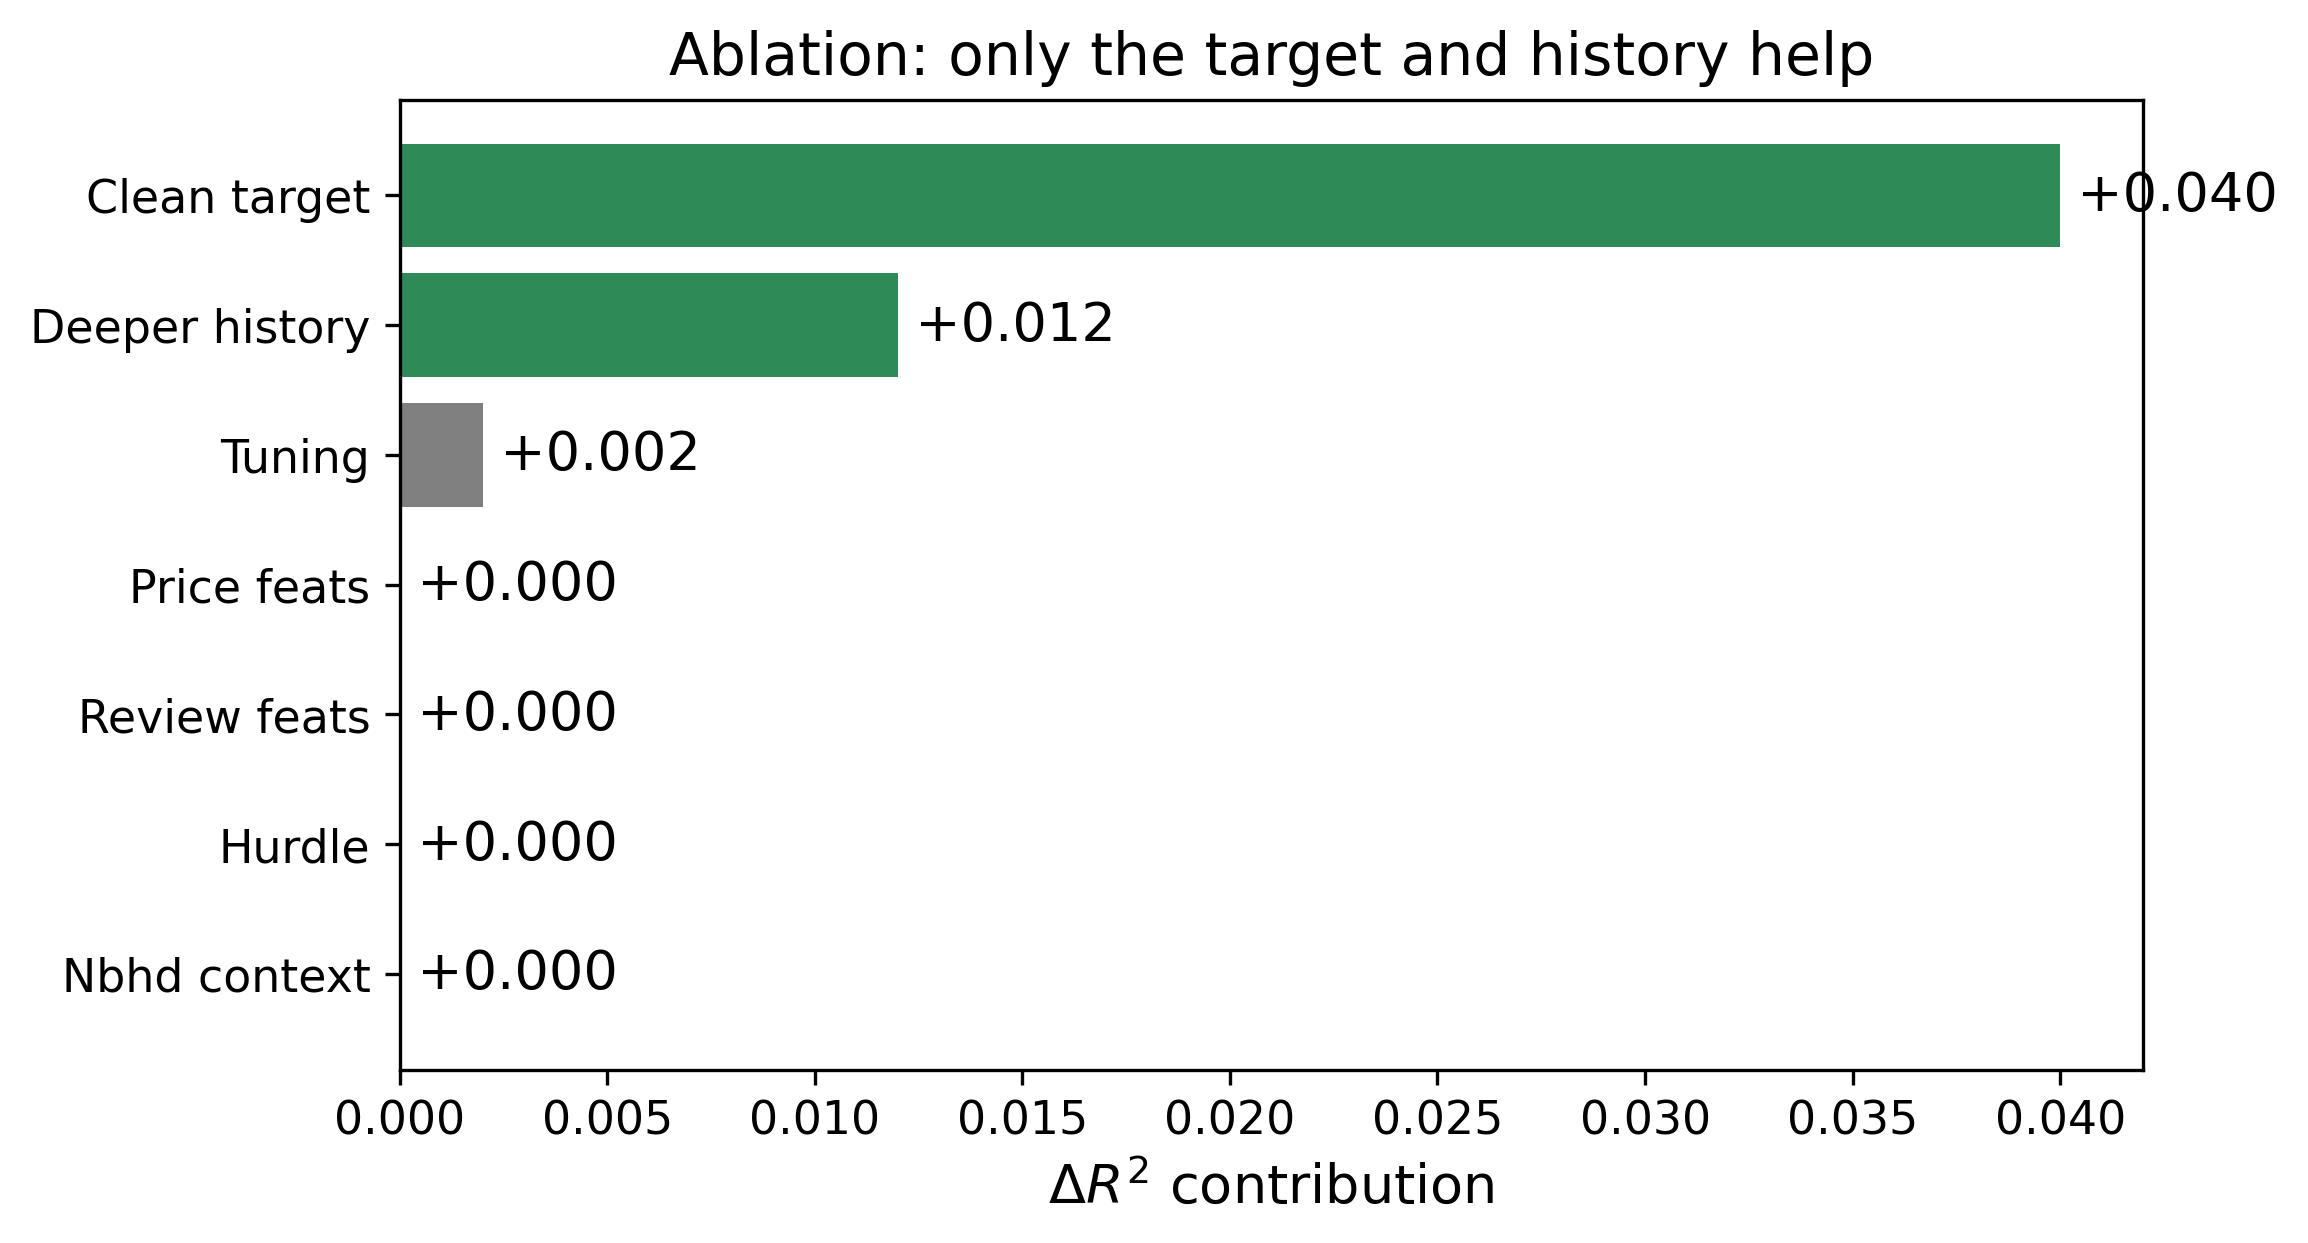
\includegraphics[width=\columnwidth]{fig6_ablation.png}
\caption{Ablation. Only the target definition and history depth contribute
meaningfully; every other component is marginal.}
\label{fig:ablation}
\end{figure}

To make the cumulative effect concrete, Table~\ref{tab:incremental} traces the
blend $R^2$ as components are added one at a time on the Q1 2026 target. The two
steps that matter---adding a second quarter of history and switching to the clean
target---together account for essentially the entire improvement, while the price
and tuning steps are flat.

\begin{table}[!t]
\caption{Cumulative ablation on the Q1 2026 target (blend $R^2$, 5-fold CV).}
\label{tab:incremental}
\centering
\small
\begin{tabular}{lcc}
\toprule
Configuration & $R^2$ & $\Delta$ \\
\midrule
Single-quarter history & 0.533 & --- \\
\quad $+$ second history quarter & 0.538 & $+0.005$ \\
\quad $+$ enriched price features & 0.537 & $-0.001$ \\
\quad $+$ clean differencing target & 0.574 & $+0.037$ \\
\quad $+$ hyper-parameter tuning & 0.576 & $+0.002$ \\
\bottomrule
\end{tabular}
\end{table}

\paragraph{Target definition (largest lever)}
Replacing the naive occupancy proxy---which is contaminated by host blocking and
is left-skewed with under $10\%$ zeros---by the clean differencing target of
\eqref{eq:booked} raises the blend $R^2$ by about $0.04$ and does so
reproducibly across periods (for Setup~A, $R^2$ rises from $0.605$ to $0.645$).
This is the single most important design choice in the paper: the bottleneck is
label quality. The mechanism behind the gain is instructive. The naive occupancy
count assigns a large value to any heavily blocked listing regardless of whether it
is actually in demand, so it forces the model to predict host calendar-management
behaviour---which is idiosyncratic and weakly related to the covariates---in
addition to demand. The differencing target strips away most of that behaviour and
leaves a signal that is far more strongly related to the listing's own history,
which the model can learn. In other words, the clean target does not make the
model smarter; it makes the quantity being predicted more predictable, by removing a
large component of essentially unlearnable variance. This reframing---that a change
of target can raise $R^2$ by making the label less noisy rather than by improving
the estimator---is, we believe, the most transferable lesson of the study for
practitioners working with indirect public data.

\paragraph{Depth of behavioural history}
Extending the history from a single quarter to two quarters, and then to seven
months, produces small but consistent gains and gives Setup~C its edge. Because the
data begin in July 2025, seven months is the deepest history available; more would
likely help further.

\paragraph{Posted price does not predict demand}
Price features were evaluated twice: a naive version sourced from months in which
the price field is empty, and a corrected version built from the months that
retain price, augmented with a neighbourhood-relative price. Neither changed the
$R^2$. In this post-regulation market, whether a listing books is governed by its
recent activity, reviews, and availability history rather than by its nightly
price---a counter-intuitive but robust negative finding. The result should not be
read as claiming that price is irrelevant to demand in general; rather, in this
data, the price that is observable is a static, host-posted asking price rather than
the realised transaction price, and it is only partially populated. Whatever
price-elasticity signal exists is evidently already reflected in the listing's
realised booking history, which the behavioural features capture directly, so the
posted price adds nothing once that history is present. This is a concrete instance
of the broader saturation phenomenon: a covariate can be correlated with demand yet
contribute no incremental predictive power when a stronger, more proximal signal is
already in the model.

\paragraph{Review velocity is redundant}
Although review recency correlates with the target ($r\approx-0.5$), adding
review-velocity features leaves the blend $R^2$ unchanged, because the
calendar-derived behavioural features already encode the same ``is this listing
active'' signal more directly. This is a clean illustration of the distinction
between marginal correlation and conditional contribution: review recency is one of
the most strongly correlated single features with the target
(Fig.~\ref{fig:review}), yet once the model already knows how many nights the
listing was booked in each recent sub-period, the additional knowledge that it was
also recently reviewed is nearly deterministic and adds no independent information.
A feature can thus be individually informative and jointly redundant, and only a
proper ablation---rather than a correlation ranking---reveals which is the case.

\paragraph{The hurdle model does not help}
On the held-out test the two-stage hurdle of \eqref{eq:hurdle} attains an $R^2$ of
$0.653$, marginally below the six-learner direct blend's $0.654$; its small
cross-validation advantage over the base blend ($+0.002$) does not survive on
unbiased data, and the hurdle formulation was not re-evaluated with the MLP
included. The gradient-boosted blend
therefore already absorbs the zero inflation as well as an explicit hurdle, and
the simpler model is preferred. This finding is worth stating carefully because the
hurdle model is often recommended almost reflexively for zero-inflated targets. Its
failure to help here does not contradict that recommendation in general; rather, it
reflects that a squared-error-optimised gradient-boosting ensemble, trained on a
target with a hard floor at zero and equipped with strong activity features, already
learns to output values very close to zero for the dormant population, so factoring
the problem explicitly buys nothing. The two-stage model would be expected to help
more under a different loss, or when the classifier and regressor can draw on
disjoint feature sets, neither of which applies here. The methodological takeaway is
to prefer the simpler direct model unless an explicit hurdle demonstrably improves a
held-out metric, which in this study it does not.

\paragraph{Feature quantity is saturated}
Neighbourhood-level demand context and explicit activity indicators added no
measurable accuracy, consistent with the general finding that once the strong
listing-level behavioural history is present, additional engineered features are
largely redundant.

Taken together, these results paint a consistent picture that is unusual to state
so plainly: the parts of the system that a practitioner would normally spend the
most effort on---model choice, hyper-parameter tuning, an explicit zero-inflation
model, and ever more elaborate feature engineering---are essentially saturated on
this problem, whereas the two decisions that are easy to overlook---how the target
is defined and how much history is used---account for virtually all of the
attainable accuracy. The practical guidance for future work on public
availability data is therefore to invest in label quality and history depth first,
and to treat additional model complexity as a last, low-yield resort. The negative
findings are as valuable as the positive one: they delineate where effort is and
is not repaid on this class of data.

%==============================================================================
\section{Limitations and Future Work}
\label{sec:limits}
Several limitations bound the present results. \emph{Label quality:} the target is
a differencing proxy that conflates guest bookings with host blocking; a cleaner
label---for instance one that fuses the availability signal with review-confirmed
occupancy---is the most promising route to higher accuracy and is left for future
work. \emph{Lost price signal:} the empty calendar price field removes a
demand-relevant covariate that cannot be recovered from this source.
\emph{Cold start:} predictions rely on behavioural history, so accuracy degrades
for brand-new listings with no calendar record. As the failure-case analysis
showed, the largest errors are concentrated precisely on listings whose
target-quarter demand decouples from their recent history---dormant properties that
suddenly fill up, or newly listed ones with no track record---and no purely
historical model can anticipate these surges from the features available. A
cold-start-aware component, perhaps drawing on neighbourhood-level demand or on the
host's other listings, is a natural remedy but lies outside the leakage-safe,
history-only framework studied here. These same failures are the dominant failure
mode in the residual analysis. \emph{Geographic and temporal scope:} the study is
confined to New York City over a ten-month window; the learned effects need not
transfer to other cities or years, and cross-city pooling is a natural extension. A further methodological caveat
concerns the target itself: because it is recovered by differencing rather than
measured, any systematic bias in how hosts manage their calendars---for instance a
tendency to block rather than un-list dates they do not intend to rent---propagates
into the label and cannot be corrected from availability data alone. Triangulating
the availability signal against the review record, and against the platform's own
trailing occupancy estimate, is a promising way to bound and reduce this bias.
Finally, the evaluation here is over listings within a fixed market; a fully
prospective evaluation, in which a model trained on one period is deployed to
forecast a strictly later one as new snapshots arrive, would be the most stringent
test of operational value and is a natural direction once a longer snapshot history
accumulates.
Finally, although the two-stage hurdle did not help here, the systematic boundary
bias in Fig.~\ref{fig:residbin} suggests that a more carefully calibrated hurdle,
or a monotone-constrained or Tweedie-loss formulation, may better handle the
extremes and merits further study. A related avenue is to model the target on a
transformed scale or with a loss matched to its count nature; the squared-error
objective used here, chosen to align with the evaluation metric, penalises the large
under-predictions of the busiest listings only in proportion to their squared
magnitude, and an asymmetric or count-aware loss might redistribute error more
favourably across the distribution. Whether any of these refinements improves a
held-out metric, rather than merely reshaping the residuals, is an empirical
question that the honest evaluation protocol established here is well suited to
answer, and which we leave to future work.

%==============================================================================
\section{Conclusion}
\label{sec:concl}
This paper presented a leakage-safe pipeline for forecasting quarterly short-term
-rental demand in New York City directly from modern, coarse public availability
snapshots. Because the Inside Airbnb calendars expose only a Boolean availability
flag and no usable price, the demand target was reconstructed by snapshot
differencing, yielding a censored, zero-inflated booking signal. A convex SLSQP
blend of six heterogeneous learners, trained on a seven-month behavioural history,
attained a $20\%$ held-out test $R^2$ of $0.654$ that closely matched its
cross-validation estimate, and its advantage over the best single learner was
statistically significant. The method proved robust across three independent
target quarters. A controlled ablation established that the dominant levers are the
target definition and the depth of behavioural history, while hyper-parameter
tuning, a two-stage hurdle model, enriched price features, review-velocity
features, and neighbourhood context each contributed little or nothing. The
practical implication is that, on this public data source, the achievable accuracy
is limited primarily by label quality---the coarse availability flag and the
missing price---rather than by model capacity, and that the most valuable direction
for improvement is a cleaner booking label rather than a more complex learner.

Beyond the specific numbers, the study offers a transferable methodology for
demand forecasting on the coarse public data that increasingly characterises the
short-term-rental domain. The snapshot-differencing target, the leakage-safe
temporal feature construction, the convex-blend combination rule, and the paired
held-out evaluation protocol are all independent of the particular city and
quarter studied here, and can be applied wherever a sequence of availability
snapshots is published. The broader lesson---that on such data the ceiling is set
by the fidelity of the recoverable label rather than by model capacity---is likely
to hold for related censored, zero-inflated forecasting problems, from parking and
venue occupancy to inventory demand, wherever the ground-truth signal must be
inferred from indirect observations rather than measured directly. We hope the
explicit reporting of what did \emph{not} help, alongside what did, provides a
useful and honest baseline for subsequent work.

A final reflection concerns the role of negative results in a field that tends to
report only improvements. Several of the design choices we examined---an explicit
hurdle stage for the zero inflation, engineered price descriptors, review-velocity
signals, and neighbourhood-level context---are individually plausible and are
routinely advocated in the literature, yet none of them moved the held-out metric
on this problem. Reporting these outcomes is not an admission of failure but a
substantive finding: it delineates, for this data source, the boundary between
model-side effort that pays and model-side effort that does not, and it redirects
future work toward the data-side interventions that our ablation identifies as the
binding constraint. We deliberately resisted the temptation to select, from among
many configurations, the single one that happened to score highest on the test
partition; the reported blend was fixed on the development data and evaluated once,
so that the headline number carries its intended meaning as an unbiased estimate of
out-of-sample accuracy rather than the maximum of a search. We regard this
discipline---fixing the model before touching the test set, and reporting the full
ledger of what helped and what did not---as the methodological core of the
contribution, and as at least as portable as the specific pipeline it produced.

In closing, we note that the practical relevance of the problem is likely to grow
rather than diminish. As platforms tighten access to granular booking data and
public-interest datasets such as Inside Airbnb increasingly become the only
window onto short-term-rental activity available to researchers, regulators, and
municipal planners, methods that extract reliable demand estimates from coarse,
availability-only snapshots acquire practical value beyond the academic. The
forecasts studied here bear directly on questions of housing supply, neighbourhood
turnover, and the regulation of whole-unit rentals, all of which depend on being
able to distinguish genuinely active listings from dormant or host-blocked ones at
scale. By documenting both the accuracy that is attainable from such data and the
precise reasons it cannot be pushed further without a cleaner label, we hope to give
practitioners a realistic basis for deciding when public snapshots suffice and when
a direct booking signal must be sought, and to give subsequent researchers a
transparent, reproducible point of departure.
\bibliographystyle{IEEEtran}
\bibliography{references}

\end{document}
